%\documentclass[10pt, twocolumn]{article}
%\documentclass[11pt]{article}
% \documentclass[twocolumn,showpacs,preprintnumbers,amsmath,amssymb,prl, superscriptaddress]{revtex4}
%\documentclass[twocolumn, preprintnumbers,amsmath,amssymb,prd, superscriptaddress]{revtex4}
\documentclass[preprintnumbers,amsmath,amssymb,prd,superscriptaddress]{revtex4}
%\documentclass[10pt, preprint,showpacs,preprintnumbers,amsmath,amssymb, superscriptaddress]{revtex4}
%\documentclass[11pt, prd,preprintnumbers,amsmath,amssymb, superscriptaddress]{revtex4}
%\documentclass[11pt, prd,preprintnumbers, amsmath,amssymb, superscriptaddress, nofootinbib, hyperref]{revtex4}

\usepackage{latexsym}
\usepackage{amssymb}
\usepackage{epsfig,amsmath,graphics}
\usepackage{epstopdf}
\usepackage{verbatim}
\usepackage{wasysym}
\usepackage{hyperref}
\usepackage{feynmp-auto} % feynman diagrams
%\usepackage{subfig}
\usepackage[utf8]{inputenc}
\usepackage{xpatch}
\usepackage{xcolor}
\usepackage{mathtools}
\hypersetup{
    colorlinks,
    linkcolor={red!80!black},
    citecolor={green!60!black},
    urlcolor={blue!60!black}}
\usepackage{appendix}

\newcommand{\Ez}{\mathcal{E}_0}
\newcommand{\Eboom}{\mathcal{E}_\text{boom}}
\newcommand{\OO}{\mathcal{O}}
\newcommand{\LL}{\mathcal{L}}
\newcommand{\HH}{\mathcal{H}}
\newcommand{\TeV}{\text{TeV}}
\newcommand{\GeV}{\text{GeV}}
\newcommand{\MeV}{\text{MeV}}
\newcommand{\keV}{\text{keV}}
\newcommand{\rad}{\text{rad}}
\newcommand{\cm}{\text{cm}}
\newcommand{\bn}{\text{b}} % barn
\newcommand{\mbn}{\text{mb}} % \millibarn
\newcommand{\angstrom}{\buildrel _{\circ} \over {\mathrm{A}}}
\newcommand{\pslash}{p\hspace{-0.070in}/\,}
\newcommand{\Mpl}{M_{\text{pl}}}
\newcommand{\ket}[1]{\ensuremath{\left|#1\right>}}
\newcommand{\bra}[1]{\ensuremath{\left<#1\right|}}
\newcommand{\braket}[2]{\ensuremath{\left<#1|#2\right>}}
\newcommand{\x}[1]{\ensuremath{\text{#1}}} % text mode shortcut
\newcommand{\kin}{\text{kin}}
\newcommand{\xmin}{\text{min}}
\newcommand{\xmax}{\text{max}}
\newcommand{\ion}{\text{ion}}
\newcommand{\TF}{\text{TF}}
\newcommand{\LPM}{\text{LPM}}
\newcommand{\el}{\text{el}}
\newcommand{\inel}{\text{inel}}
%Large Parentheses
\def\r{\right)}
\def\l{\left(}

\newcommand{\overbar}[1]{\mkern 1.5mu\overline{\mkern-1.5mu#1\mkern-1.5mu}\mkern 1.5mu}

\begin{document}

%\preprint{APS/123-QED}

\title{White Dwarfs as Dark Matter Detectors}

\author{Peter W. Graham}
\affiliation{Stanford Institute for Theoretical Physics, Department of Physics,
Stanford University, Stanford, CA, 94305}

\author{Ryan Janish}
\affiliation{Berkeley Center for Theoretical Physics, Department of Physics,
University of California, Berkeley, CA 94720, USA}

\author{Vijay Narayan}
\affiliation{Berkeley Center for Theoretical Physics, Department of Physics,
University of California, Berkeley, CA 94720, USA}

\author{Surjeet Rajendran}
\affiliation{Berkeley Center for Theoretical Physics, Department of Physics,
University of California, Berkeley, CA 94720, USA}

\author{Paul Riggins}
\affiliation{Berkeley Center for Theoretical Physics, Department of Physics,
University of California, Berkeley, CA 94720, USA}

\begin{abstract}
Dark matter that is capable of sufficiently heating a local region in a white dwarf will trigger runaway fusion and ignite a type Ia supernova.
This was originally proposed in~\cite{Graham:2015apa} and used to constrain primordial black holes which transit and heat a white dwarf via dynamical friction.
In this paper, we consider dark matter (DM) candidates that heat through the production of high-energy standard model (SM) particles, and show that such particles will efficiently thermalize the white dwarf medium and ignite supernovae.
Based on the existence of long-lived white dwarfs and the observed supernovae rate, we derive new constraints on ultra-heavy DM which produce SM particles through DM-DM annihilations, DM decays, and DM-SM scattering interactions in the stellar medium. 
As a concrete example, we rule out supersymmetric Q-ball DM in parameter space complementary to terrestrial bounds.
We put further constraints on DM that is captured by white dwarfs, considering the formation and self-gravitational collapse of a DM core which heats the star via decays and annihilations within the core.
It is also intriguing that the DM-induced ignition discussed in this work provide an alternative mechanism of triggering supernovae from sub-Chandrasekhar, non-binary progenitors.
\end{abstract}

\maketitle

%%%%%%%%%%%%%%%%%%%%%%%%%%%%%%%%%%%%%%%%%%%%%%%%%%%%%%%%%%%%%%%%
\section{Introduction}
\label{sec:intro}
Identifying the nature of dark matter (DM) remains one of the clearest paths beyond the Standard Model (SM) and it is thus fruitful to study the observable signatures of any yet-allowed DM candidate.
Many direct detection experiments are designed to search for DM, e.g.~\cite{Akerib:2016vxi, Agnese:2017njq}, yet these lose sensitivity to heavier DM due to its diminished number density.
Even for a strongly-interacting candidate, if the DM mass is above $\sim 10^{22}~\GeV$ a terrestrial detector of size $\sim (100~\text{m})^2$ will register fewer than one event per year.
While these masses are large compared to those of fundamental particles, it is reasonable to suppose that DM may exist as composite states just as the SM produces complex structures with mass much larger than fundamental scales (e.g., you, dear reader).
Currently there is a wide range of unexplored parameter space for DM candidates less than $\sim 10^{48}~\GeV$, above which the DM will have observable gravitational microlensing effects~\cite{Griest:2013aaa}.
For such ultra-heavy DM, indirect signatures in astrophysical systems are a natural way forward.
One such signal, proposed by~\cite{Graham:2015apa}, is that DM can trigger runaway fusion and ignite type Ia supernovae (SN) in sub-Chandrasekhar white dwarf (WD) stars.

In addition to constraining the properties of DM, this raises the intriguing possibility that DM-induced runaway fusion is responsible for a fraction of the observed astrophysical transients. 
The progenitors of type Ia SN are not fully understood~\cite{
Maoz:2012}, and recent observations of sub-Chandrasekhar~\cite{Scalzo:2014sap, Scalzo:2014wxa}, hostless~\cite{McGee:2010}, and unusual type Ias~\cite{Foley:2013} suggest that multiple progenitor systems and ignition mechanisms are operative.
Other suspected WD thermonuclear events, such as the Ca-rich transients~\cite{Kasliwal:2012}, are also poorly understood. 
While mechanisms for these events have been proposed~\cite{Woosley1994,Fink:2007fv,Pakmor:2013wia,Sell:2015rfa}, the situation is yet unclear and it is worthwhile to consider new sources of thermonuclear ignition. 

Runaway thermonuclear fusion requires both a heating event and the lack of significant cooling which might quench the process.
The WD medium is particularly suited to this as it is dominated by degeneracy pressure and undergoes minimal thermal expansion, which is the mechanism that regulates fusion in main sequence stars.
Thermal diffusion is the primary cooling process in a WD and it can be thwarted by heating a large enough region.
The properties of a localized heating necessary to trigger runaway fusion were computed in~\cite{Woosley}.
Consequently, it was realized~\cite{Graham:2015apa} that if DM is capable of sufficiently heating a WD in this manner, it will result in a SN with sub-Chandrasekhar mass progenitor.
This was used to constrain primordial black holes which transit a WD and cause heating by dynamical friction, although the authors of~\cite{Graham:2015apa} identify several other heating mechanisms which may be similarly constrained.

In this paper, we examine DM candidates with non-gravitational interactions that cause heating through the production of SM particles.
An essential ingredient in this analysis is understanding the length scales over which SM particles deposit energy in a WD medium.
We find that most high energy particles thermalize rapidly, over distances shorter than or of order the critical size for fusion. 
Particle production is thus an effective means of igniting WDs. 
Constraints on these DM candidates come from either observing specific, long-lived WDs or by comparing the measured rate of type Ia SN with that expected due to DM.
It is important to note that these constraints are complementary to direct searches---it is more massive DM that is likely to trigger SN, but also more massive DM that has low terrestrial flux.
The WD detector excels in this regime due to its large surface area $\sim (10^4~\text{km})^2$, long lifetime $\sim \text{Gyr}$, and high density. 
We demonstrate these constraints for generic classes of DM models that produce SM particles via DM-SM scattering, DM-DM collisions, or DM decays, and consider the significantly enhanced constraints for DM that is captured in the star.
As a concrete example we consider ultra-heavy Q-ball DM as found in supersymmetric extensions of the SM. 

The rest of the paper is organized as follows.
We begin in Section~\ref{sec:boomreview} by reviewing the mechanism of runaway fusion in a WD.
In Section~\ref{sec:smheating} we study the heating of a WD due to the production of high-energy SM particles.
Detailed calculations of the stopping of such particles are provided in Appendix~\ref{sec:wdpdg}.
In Section~\ref{sec:dmignition} we parameterize the explosiveness and event rate for generic classes of DM-WD encounters, and in Section~\ref{sec:constraints} we derive schematic constraints on such models.
The details of DM capture in a WD are reserved for Appendix~\ref{sec:capture}.
Finally we specialize to the case of Q-balls in Section~\ref{sec:qballs}, and conclude in Section~\ref{sec:discussion}.

%%%%%%%%%%%%%%%%%%%%%%%%%%%%%%%%%%%%%%%%%%%%%%%%%%%%%%%%%%%%%%%%
\section{White Dwarf Runaway Fusion}
\label{sec:boomreview}
We first review the conditions for which a local energy deposition in a WD results in runaway fusion.
Any energy deposit will eventually heat ions within some localized region---parameterize this region by its linear size $L_0$, total kinetic energy $\Ez$ and typical temperature $T_0$.
These scales evolve in time, but it will be useful to describe a given heating event by their initial values.

The fate of a heated region is either a nonviolent diffusion of the excess energy across the star, or a runaway fusion chain-reaction that destroys the star.
The precise outcome depends on $L_0$, $\Ez$ and $T_0$.
There is a critical temperature $T_f$, set by the energy required for ions to overcome their mutual Coulomb barrier, above which fusion occurs.
For carbon burning, $T_f \sim \MeV$~\cite{Gasques:2005ar}.
Any heated region $T_0 > T_f$ will initially support fusion, although this is not sufficient for runaway as cooling processes may rapidly lower the temperature below $T_f$.
This cooling will not occur if the corresponding timescale is larger than the timescale at which fusion releases energy.
Cooling in a WD is dominated by thermal diffusion, and the diffusion time increases as the size of the heated region.
However, the timescale for heating due to fusion is independent of region size.
Thus, for a region at temperature $\gtrsim T_f$, there is a critical size above which the heated region does not cool but instead initiates runaway.
For a region at the critical fusion temperature $T_f$, we call this critical size the \emph{trigger size} $\lambda_T$.
The value of $\lambda_T$ is highly dependent on density, and in a WD is set by the thermal diffusivity of either photons or degenerate electrons.
This critical length scale has been computed numerically in~\cite{Woosley} for a narrow range of WD densities and analytically scaled for other WD masses in~\cite{Graham:2015apa}.
As in~\cite{Graham:2015apa}, we will restrict our attention to carbon-oxygen WDs in the upper mass range $\sim 0.85 - 1.4 ~M_{\astrosun}$ (these will yield the most stringent constraints on DM).
This corresponds to a central number density of ions $n_\text{ion} \sim 10^{30} - 10^{32} ~\cm^{-3}$ and a trigger size of $\lambda_T \sim 10^{-3} - 10^{-5} ~\text{cm}$.

If a heated region is smaller than the trigger size, its thermal evolution is initially dominated by diffusion.
However, this will still result in runaway fusion if the temperature is of order $T_f$ by the time the region diffuses out to the trigger size.
For our purposes it is more natural to phrase this in terms of the total energy $\Ez$ deposited during a heating event.
Of course, the relation between energy $\Ez$ and temperature $T_0$ depends on the rate at which WD constituents---ions, electrons, and photons---thermalize with each other within the region size $L_0$.
Given that the different species thermalize rapidly, the excess energy required to raise the temperature to $T_f$ in a volume $V$ is given by a sum of their heat capacities
\begin{equation}
\label{eq:heatcapacity}
  \frac{\Ez}{V} \gtrsim \int_0^{T_f} dT (n_\text{ion} + n_e^{2/3} T + T^3),
\end{equation}
where $n_e$ is the number density of electrons.
Note that we use the heat capacity of a degenerate gas of electrons, since the Fermi energy $E_F \gtrsim \MeV$ for the densities we consider.
The minimum energy deposit necessary to trigger runaway fusion is simply
\begin{align}
\label{eq:Eboom}
\Eboom &\sim \lambda_T^3 (n_\text{ion} T_f + n_e^{2/3} T_f^2 + T_f^4) \\
&\approx 10^{16} - 10^{23} ~\GeV. \nonumber
\end{align}
$\Eboom$ varies with $\lambda_T$ over the range of WD densities and is plotted in Figure~\ref{fig:Eboom}.
Thus for a heating event characterized by its $L_0$, $\Ez$, and $T_0 \gtrsim T_f$, there is an \emph{ignition condition}:
\begin{align}
    \label{eq:energy_boom_condition}
    \Ez \gtrsim
    \Eboom \cdot \text{max}\left\{1, \frac{L_0}{\lambda_T}\right\}^3.
\end{align}
Any $\Ez$ satisfying this condition is minimized for $L_0$ less than the trigger size, where it is also independent of the precise value of $L_0$.
For broader deposits, the necessary energy is parametrically larger than $\Eboom$ by a volume ratio $(L_0/\lambda_T)^3$.
As a result, understanding the $L_0$ for different kinds of heating events in a WD is critical to determining whether or not they are capable of destroying the star.

\begin{figure}
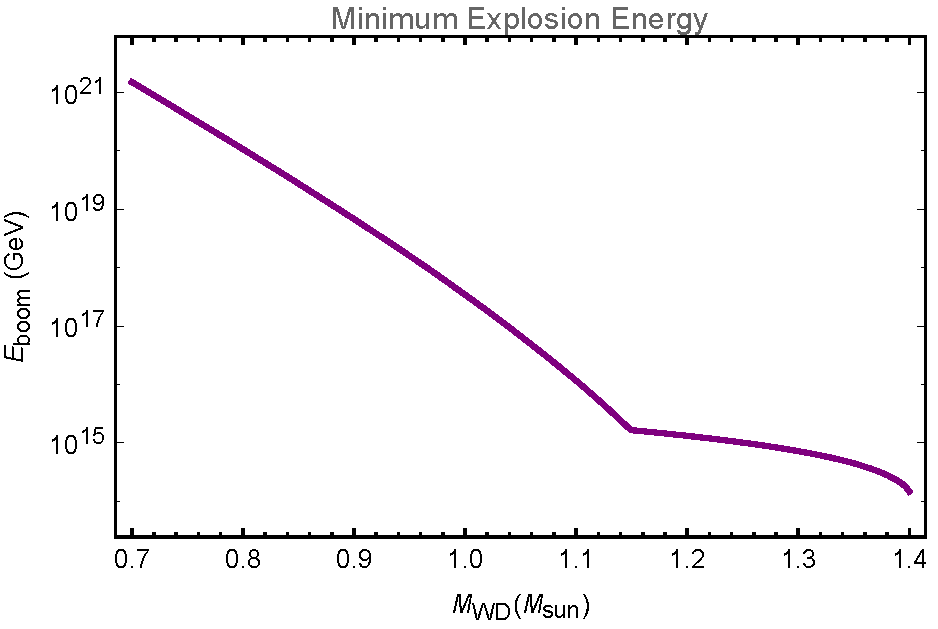
\includegraphics[scale=.35]{Eboom.pdf}
\caption{The minimum energy deposit~\eqref{eq:Eboom} necessary to trigger runaway fusion, based on numerical results for $\lambda_T$~\cite{Woosley} and the WD mass-density relation~\cite{cococubed}}.
\label{fig:Eboom}
\end{figure}


%%%%%%%%%%%%%%%%%%%%%%%%%%%%%%%%%%%%%%%%%%%%%%%%%%%%%%%%%%%%%%%%
\section{Particle Heating of White Dwarfs}
\label{sec:smheating}
% !TEX root = wd-full.tex

Production of high-energy SM particles in a WD will result in heating of the stellar medium.
The critical quantity to understand is the length scale over which such heating occurs---this scale determines the efficiency of the heating event in triggering runaway fusion, as described by condition~\eqref{eq:energy_boom_condition}.
Note that this is a question of purely SM physics.
The unknown physics of DM will serve only to set the initial properties of the SM particles.

We find that SM particles efficiently heat the WD regardless of species or energy (neutrinos are a slight exception)---the heating length is typically less than or of order the trigger size $\lambda_T$.
This is accomplished primarily through hadronic showers initiated by collisions with carbon ions.
In some cases electromagnetic showers are important, however at high energies these are suppressed by density effects and even photons and electrons are dominated by hadronic interactions.
These showers rapidly stop high-energy particles due to their logarithmic nature, transferring the energy into a cloud of low-energy particles which heat the medium through elastic scatters.
A schematic for the flow of energy during deposition is given in Figure~\ref{fig:cooling-cartoon}.
In this light, the WD operates analogously to a particle detector, including hadronic and electromagnetic ``calorimeter'' components.
Runaway fusion provides the necessary amplification to convert a detected event into an observable signal.

\begin{figure*}
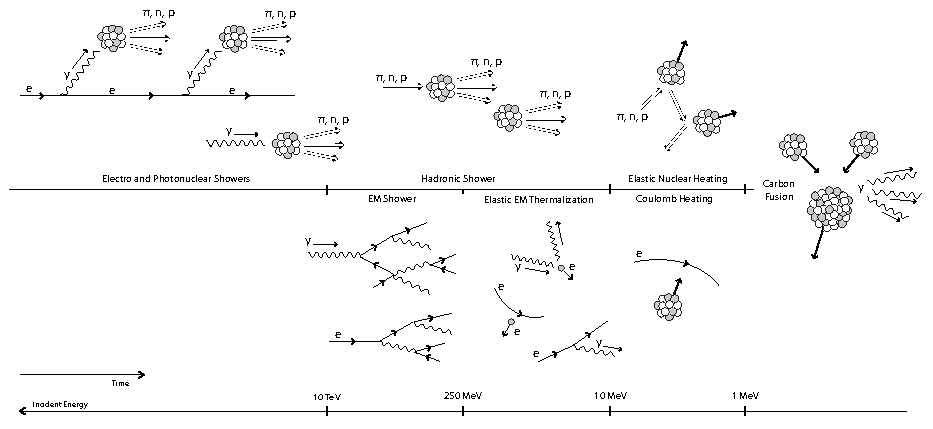
\includegraphics[scale=1.15]{cooling-cartoon.pdf}
\caption{Dominant energy loss and thermalization processes in the WD as a function of energy, with energy decreasing towards the right.
Hadronic processes are shown in the upper panel and EM processes in the lower panel.
High energy particles will induce showers that terminate into elastic thermalization of the WD ions, moving from left to right in the diagram.
The quoted energies are for a $\sim 1.37 ~M_{\astrosun}$ WD, although the cartoon is qualitatively the same for all densities.}
\label{fig:cooling-cartoon}
\end{figure*}


The remainder of this section will discuss the above heating process in more detail.
We summarize the dominant source of energy loss and the resulting stopping lengths $\lambda$ for SM particles of incident kinetic energy $\epsilon$.
The total path length traveled by a particle before depositing $\OO(1)$ of its energy is approximately
\begin{equation}
R_\text{SP} \sim \frac{\epsilon}{dE/dx},
\end{equation}
where $dE/dx$ is the stopping power in the WD medium.
If the mean free path to hard scatter $\lambda_\text{hard}$ is smaller than this path length $R_\text{SP}$, then the particle undergoes a random walk with $N_\text{hard}$ scatters, and the net displacement is reduced by $\sqrt{N_\text{hard}}$.
We therefore approximate the stopping length as
\begin{align}
\lambda \sim \text{min}\left\{ R_\text{SP}, \sqrt{R_\text{SP}\lambda_\text{hard}} \right\}
\end{align}
This random walk behavior is relevant for low-energy elastic scatters.

Stopping lengths are plotted in Figures~\ref{fig:SPhighHad} and~\ref{fig:SPhighEM}, and a detailed treatment of the stopping powers is given in Appendix~\ref{sec:wdpdg}.
We will consider incident light hadrons, photons, electrons, and neutrinos---as we are concerned with triggering runaway fusion, we restrict our attention to energies $\epsilon \gg T_f \sim \text{MeV}$.


\subsection{High-Energy Showers}

\paragraph{Hadronic Showers.}
Incident hadrons with kinetic energy larger than the nuclear binding scale $\sim 10~\MeV$ will undergo violent inelastic collisions with carbon ions resulting in an $\OO(1)$ number of secondary hadrons.
This results in a roughly collinear shower of hadrons of size
\begin{align}
\label{eq:hadlength}
  X_\text{had} &\sim \frac{1}{n_\ion \sigma_\text{inel}} \log\l\frac{\epsilon}{10 ~\MeV}\r \\
  &\approx 10^{-6} ~\text{cm}
  \l\frac{10^{32}~\text{cm}^{-3}}{n_\text{ion}}\r. \nonumber
\end{align}
where the inelastic nuclear cross section is $\sigma_\text{inel} \approx 100 ~\text{mb}$ and we have taken the logarithm to be $\sim 10$.
The shower terminates into pions and nucleons of energy $\sim 10~\MeV$, whose cooling is discussed below.
Note that neutral pions of energy $10 - 100 ~\text{MeV}$ have a decay length to photons of $\delta_{\pi^0} \sim 10^{-6} ~\text{cm}$.
Hadronic showers will therefore generate an electromagnetic component carrying an $\OO(1)$ fraction of the energy.

\begin{figure}
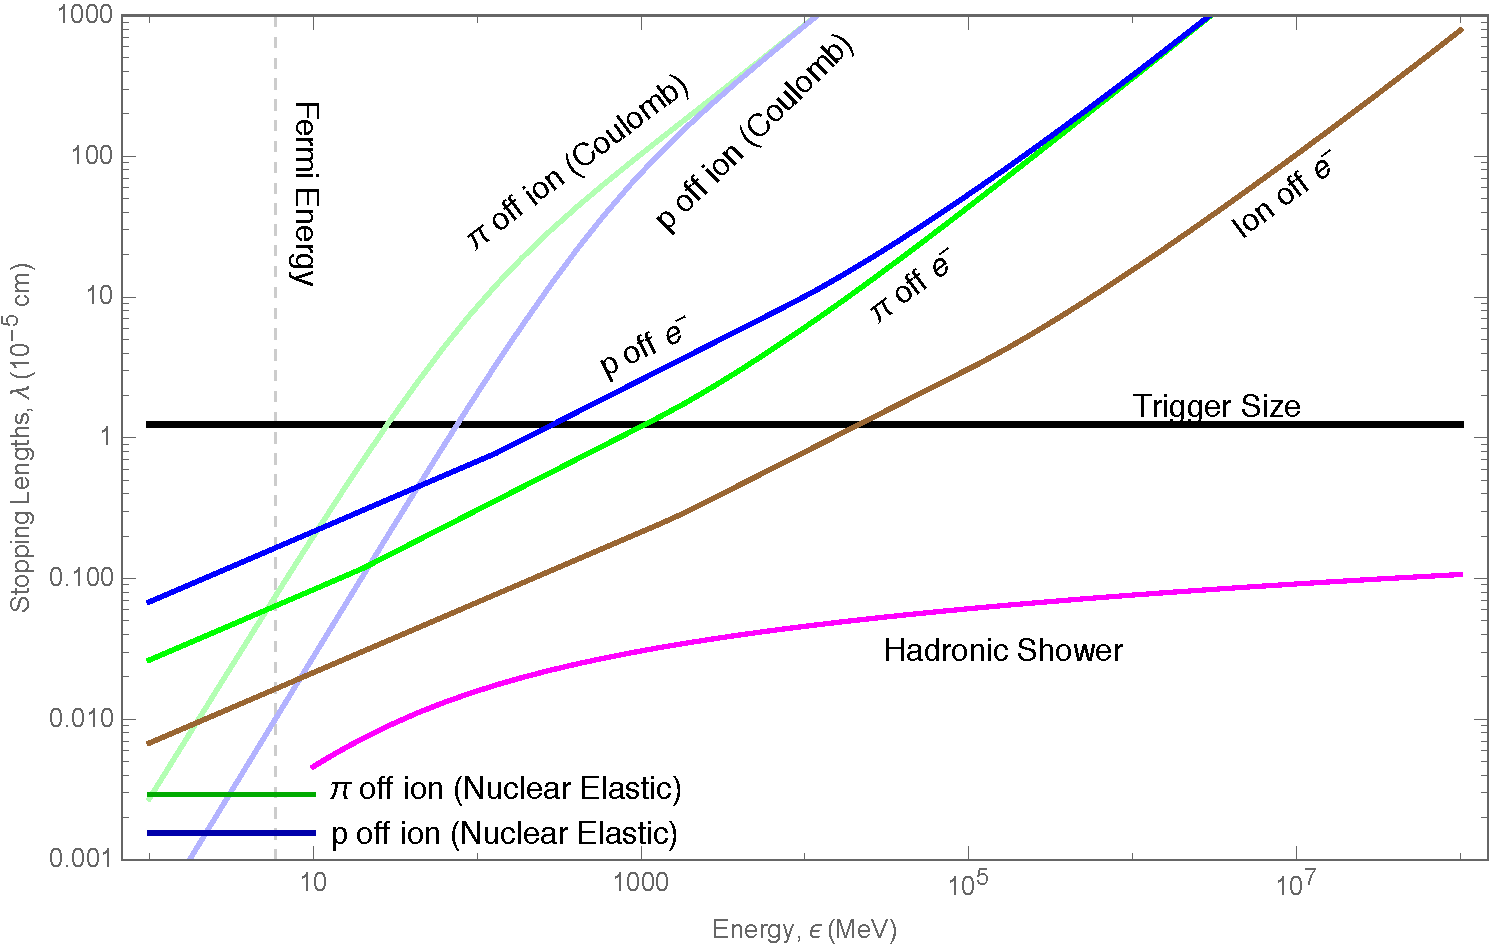
\includegraphics[scale=.35]{SPhighHad.pdf}
\caption{Stopping lengths for incident hadrons as a function of kinetic energy in a WD of density $n_\text{ion} \sim 10^{31}~\text{cm}^{-3}$ ($\approx 1.25 ~M_{\astrosun}$), including the hadronic shower length (magenta).
Any discontinuities in the stopping lengths are due to approximate analytic results in the different energy regimes.
See Appendix~\ref{sec:wdpdg} for calculation details.
}
\label{fig:SPhighHad}
\end{figure}

\begin{figure}
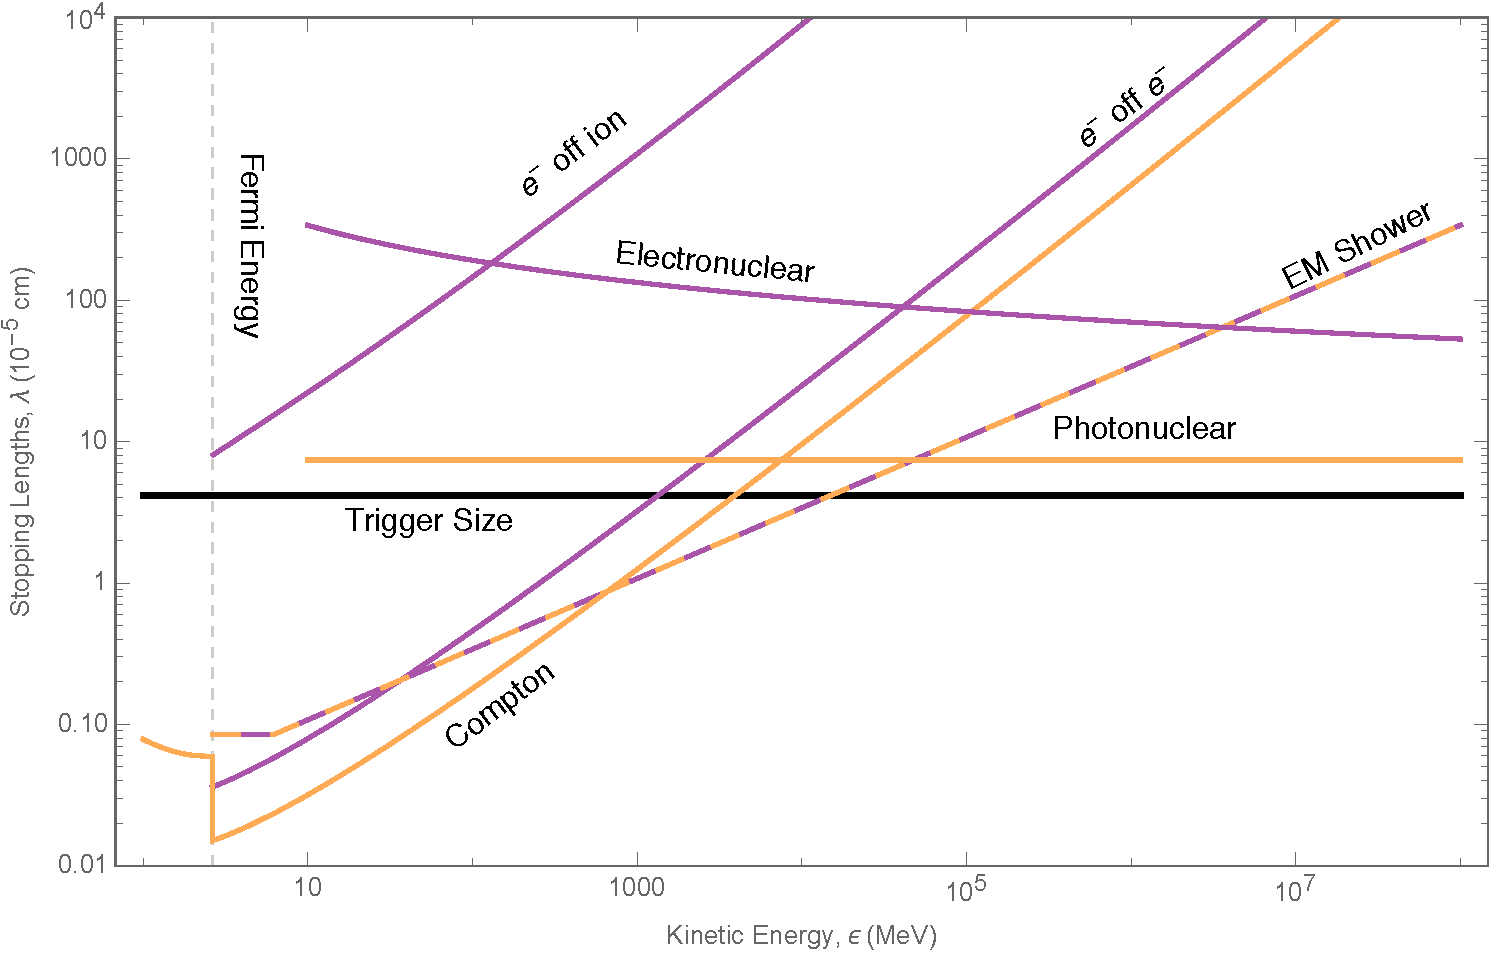
\includegraphics[scale=.35]{SPhighEM.pdf}
\caption{Stopping lengths of incident photons (orange) and electrons (purple) as a function of kinetic energy in a WD of density $n_\text{ion} \sim 10^{31}~\text{cm}^{-3}$ ($\approx 1.25 ~M_{\astrosun}$), including the EM shower length (dashed).
Any discontinuities in the stopping lengths are due to approximate analytic results in the different energy regimes.
See Appendix~\ref{sec:wdpdg} for calculation details.
}
\label{fig:SPhighEM}
\end{figure}


\paragraph{Photonuclear and Electronuclear Showers.}
A photon or electron can directly induce hadronic showers via production of a quark-antiquark pair, depicted in Figure~\ref{fig:electrophotonuclear-diagram}.
The LPM effect, discussed below, ensures that these process dominate the stopping of photons and electrons at high energies, $\epsilon \gtrsim 10^4-10^6~\GeV$.

\begin{figure}
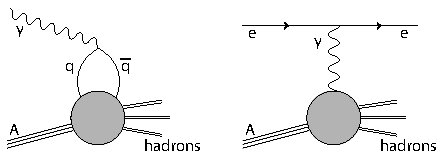
\includegraphics[scale=1.0]{electrophotonuclear-diagram.pdf}
\caption{Photonuclear (left) and Electronuclear (right) interactions. The shaded region contains, at high energies, the familiar point-like processes of deep inelastic scattering and for energies below $\Lambda_\x{QCD}$ is best described by exchange of virtual mesons.}
\label{fig:electrophotonuclear-diagram}
\end{figure}

The only substantial difference between photonuclear showers and purely hadronic ones is that they require a longer distance to initiate.
Roughly, the photonuclear cross section is suppressed relative to the hadronic inelastic cross section $\sigma_\text{inel}$ by a factor of $\alpha$, and so the photon range is
\begin{align}
\label{eq:photonuclength}
  \lambda_{\gamma A} \approx 10^{-5} ~\text{cm} \l\frac{10^{32}~\text{cm}^{-3}}{n_\text{ion}}\r.
\end{align}
Here $\lambda_{\gamma A}$ is the distance to initiate a hadronic shower, whereas the shower itself extends a distance $X_\text{had}$.
Note that $\lambda_{\gamma A}$ is of order the trigger size.

The electronuclear showers are qualitatively different, as the electron survives the interaction.
This process is best described as a continuous energy loss of the electron, due to radiation of virtual photons into hadronic showers.
The stopping power is again radiative, which gives the constant stopping length
\begin{align}
\label{eq:electronuclength}
  \lambda_{eA}
  \approx 10^{-4} ~\text{cm} \l\frac{10^{32}~\text{cm}^{-3}}{n_\text{ion}}\r.
\end{align}
This is suppressed by an additional factor of $\alpha$ relative to the photonuclear interaction, although a full calculation also yields an $\OO(10)$ logarithmic enhancement.
We see that the electronuclear length scale $\lambda_{eA}$ is at most larger than the trigger size by an order of magnitude.

\paragraph{Electromagnetic Showers.}
Of course, electrons and photons can also shower through successive bremsstrahlung and pair-production.
An electromagnetic shower proceeds until a critical energy $\sim 100 ~\MeV$, at which point these radiative processes become subdominant to elastic Coulomb and Compton scattering.
Below this scale radiation can still be important, though electromagnetic showers do not occur.
Note that bremsstrahlung and pair-production are strictly forbidden for incident energies below the Fermi energy $E_F$.

At sufficiently high electron/photon energies and nuclear target densities, electromagnetic showers are elongated due to the Landau-Pomeranchuk-Migdal (LPM) effect.
High-energy radiative processes necessarily involve small momentum transfers to nuclei.
These soft virtual photons cannot be exchanged with only a single ion, but rather interact simultaneously with multiple ions.
This generates a decoherence, suppressing bremsstrahlung/pair-production above an energy $E_\text{LPM}$ which scales inversely with density:
\begin{align}
    E_\text{LPM} \approx 1~\MeV
    \l \frac{10^{32}~\text{cm}^{-3}}{n_\text{ion}} \r
\end{align}
The corresponding shower lengths are
\begin{align}
  X_\text{EM} &\approx X_0 \cdot
  \begin{cases}
  \l \frac{\epsilon}{E_\text{LPM}} \r^{1/2} & \epsilon > E_\text{LPM} \\
  \;\;\;\;\;\, 1 & \epsilon < E_\text{LPM}
  \end{cases}
\end{align}
where
\begin{align}
  X_0 &\approx 10^{-7} ~\text{cm}
  \l\frac{10^{32}~\text{cm}^{-3}}{n_\text{ion}}\r.
\end{align}
is the unsuppressed EM shower length.
See Appendix~\ref{sec:emshowers} for details.
At the highest WD densities radiative processes are always LPM-suppressed, while at lower densities we observe both regimes.
We emphasize that for all densities, throughout the energy range where it is relevant, the length of electromagnetic showers is never parametrically larger than the trigger size.

\paragraph{Neutrinos.}
Neutrinos scatter off nuclei with a cross section that increases with energy.
In these interactions, an $\OO(1)$ fraction of the neutrino energy is transferred to the nucleus with the rest going to produced leptons---this is sufficient to start a hadronic shower \cite{Gandhi:1998ri, Formaggio:2013kya}.
At an energy of $\sim 10^{11} ~\GeV$, \cite{Gandhi:1998ri} calculates the neutrino-nuclear cross section to be $\sim 10^{-32} ~\cm^2$.
Conservatively assuming this value for even higher energies, we find a neutrino mean free path in a WD of order $\sim 10 ~\cm$.
While this distance is much too large to heat a WD via the release of multiple low-energy neutrinos, for a single neutrino it is simply a displacement after which a compact shower of size $X_\text{had}$ occurs.
As such, a \emph{single} high-energy neutrino will heat the star just as high-energy hadrons do.

\subsection{Low-Energy Elastic Heating}
The showers of high-energy particles described above terminate in a cloud of low-energy $\epsilon \sim 10~\MeV$ neutrons, protons, and charged pions, and $\epsilon \sim 10-100~\MeV$ electrons and photons.
Of course, particles at these energies may also be directly produced by the DM.
At these energies, elastic nuclear, Coulomb, and Compton scatters dominate and eventually lead to the thermalization of ions.

\paragraph{Hadrons.}
Neutral hadrons are the simplest species we consider, interacting at low-energies only through elastic nuclear scatters with cross section $\sigma_\text{el} \approx \text{b}$.
Note that the large ion mass requires $\sim 10 - 100$ hard scatters to transfer the hadron's energy in the form of a random-walk.
This elastic heating range is
\begin{align}
 \lambda_\text{el} &\approx
 10^{-7} ~\text{cm} \l\frac{10^{32}~\text{cm}^{-3}}{n_\text{ion}}\r,
\end{align}
and is always less than the trigger size.

Charged hadrons are also subject to Coulomb interactions, which would provide the dominant stopping in terrestrial detectors.
In this case, however, Coulomb scatters off degenerate WD electrons are strongly suppressed and charged hadrons predominantly undergo elastic nuclear scatters like their neutral brethren.
This suppression is due to (1) motion of the electrons, which fixes the relative velocity to be $\OO(1)$ and removes the enhancement of Coulomb stopping usually seen at low velocity, and (2) Pauli blocking, which forces the incident particle to scatter only electrons near the top of the Fermi sea.
For an incident particle with velocity $v_\x{in} \ll 1$, the first effect suppresses the stopping power by a factor of $v_\x{in}^2$ relative to that off stationary, non-degenerate electrons and the second by an additional factor of $v_\x{in}$.
Note that there is a small range of energies in which Coulomb scatters off ions dominate the stopping of charged hadrons---either way, both length scales are well below the trigger size.

\paragraph{Electrons and Photons.}
For electrons and photons below $\sim 100 ~\MeV$ the dominant interactions are Coulomb scatters off WD electrons and Compton scatters, respectively.
The length scale of these processes is smaller than any interaction with ions, and so these electrons and photons will thermalize into a compact electromagnetic ``gas" with a size set by the radiative length scale $X_\text{EM}$.
The EM gas will cool and diffuse to larger length scales, eventually allowing thermalization with nuclei via the subdominant Coulomb scatters of electrons off ions.
The photons of the EM gas will not undergo photonuclear showers here, as the gas will cool below $\sim 10~\MeV$ by the time it diffuses out to a size $\lambda_{\gamma A}$.
This gas temperature is initially at most $\sim 100~\MeV$.
At these temperatures the heat capacity is dominated by photons, so as the gas diffuses to a size $\lambda_{\gamma A}$ it cools by a factor $(X_\text{EM}/\lambda_{\gamma A})^{3/4} \sim 10^{-2} - 10^{-1}$.
Note that for temperatures $T$ less than $E_F$, the electrons are partially degenerate and heating proceeds via the thermal tail with kinetic energies $\epsilon \sim E_F + T$.
Therefore, the relevant thermalization process is Coulomb scattering of electrons off ions.

Like the hadronic elastic scatters, an electron Coulomb scattering off ions will occasionally hard scatter, and thus deposit its energy along a random walk. This reduces the stopping length at low energies, yielding
\begin{equation}
\lambda_\text{coul} \approx 10^{-6}~\cm \l \frac{\epsilon}{10 ~\MeV} \r^{3/2} \l \frac{10^{32} ~\cm^{-3}}{n_\text{ion}}\r
\end{equation}
which is below the trigger size.


%%%%%%%%%%%%%%%%%%%%%%%%%%%%%%%%%%%%%%%%%%%%%%%%%%%%%%%%%%%%%%%%
\section{Dark Matter-Induced Ignition}
\label{sec:dmignition}
% !TEX root = wd-full.tex

Any DM interaction that produces SM particles in a WD has the potential to ignite the star, provided that sufficient SM energy is produced.
The distribution in space, momentum, and species of these SM products is dependent on unknown DM physics and is needed to determine the rate of DM-induced ignition.
This can be done precisely for a specific DM model, as we do for Q-balls in Section~\ref{sec:qballs}.
In this Section, however, we study some general features of DM-WD encounters involving DM that possesses interactions with itself and the SM.
We collect below the basic formulas relating DM model parameters to ignition criteria, SN rate, etc.

DM can generically heat a WD through three basic processes: DM-SM scattering, DM-DM collisions, and DM decays.
For ultra-heavy DM, these processes can be complicated events involving many (possibly dark) final states, analogous to the interactions of heavy nuclei.
In the case of DM-SM scattering, we consider both elastic and inelastic DM scatters off WD constituents, e.g.~carbon ions.
We classify DM candidates into three types according to the interaction that provides the dominant source of heating, and refer to these as scattering, collision, and decay candidates.
We also make the simplifying assumption that the above events are ``point-like", producing SM products in a localized region (smaller than the heating length) near the interaction vertex.
Where this is not the case (as in our elastic scattering and Q-ball constraints, see Sections~\ref{sec:TransitConstraints} and~\ref{sec:qballs}), then the same formalism applies but with the event size added to the stopping length.

The SN rate may be greatly enhanced if DM is captured in the star, so we also consider separately ``transiting DM" and ``captured DM".
In general, there is some loss of DM kinetic energy in the WD.
In the transit scenario, this energy loss is negligible and the DM simply passes through the star.
In the capture scenario, the energy loss is not directly capable of ignition but is sufficient to stop the DM and cause it to accumulate in the star.
Energy loss may be due to a variety of processes, but for simplicity we will focus on an DM-nuclei elastic scattering.
Of course, due to the velocity spread of DM in the rest frame of a WD, there will necessarily be both transiting and captured DM populations in the star.

\subsection{DM Transit}

\paragraph{DM-SM Scattering.}
Runaway fusion only occurs in the degenerate WD interior where thermal expansion is suppressed as a cooling mechanism.
The outer layers of the WD, however, are composed of a non-degenerate gas and it is therefore essential that a DM candidate penetrate this layer in order to ignite a SN.
We parameterize this by a DM stopping power $(dE/dx)_\text{SP}$, the kinetic energy lost by the DM per distance traveled in the non-degenerate layer, and demand that
\begin{align}
\label{eq:CrustCondition}
  \left( \frac{d E}{d x} \right)_\text{SP} \ll
  \frac{m_\chi v^2_\text{esc}}{R_\text{env}},
\end{align}
where $R_\text{env}$ is the nominal size of the non-degenerate WD envelope and $v_\text{esc} \sim 10^{-2}$ is the escape velocity of the WD, at which the DM typically transits the star. 

DM-SM scattering will result in a continuous energy deposit along the DM trajectory (if the interaction is rare enough for this not to be true, then the encounter is analogous to the case of DM decay).
This is best described by a linear energy transfer $(dE/dx)_\text{LET}$, the kinetic energy of SM particles produced per distance traveled by the DM.
If these products have a heating length $L_0$ then the energy deposit must at minimum be taken as the energy transferred along a distance $L_0$ of the DM trajectory.
Importantly, as per the ignition condition~\eqref{eq:energy_boom_condition}, such a deposition is \emph{less} explosive unless $L_0$ is smaller than the trigger size $\lambda_T$.
We thus consider the energy deposited over the larger of these two length scales.
Assuming the energy of the DM is roughly constant during this heating event, the ignition condition is:
\begin{align}
\label{eq:transitexplosion}
  \left( \frac{d E}{d x} \right)_\text{LET} \gtrsim
  \frac{\Eboom}{\lambda_T} \cdot \text{max}
  \left\{\frac{L_0}{\lambda_T}, 1 \right\}^2.
\end{align}
Note that the DM stopping power $(dE/dx)_\text{SP}$ and the linear energy transfer $(dE/dx)_\text{LET}$ are related in the case of elastic scatters, but in general the two quantities may be controlled by different physics.
In addition, a transit event satisfying condition~\eqref{eq:CrustCondition} will have negligible energy loss over the parametrically smaller distances $\lambda_T$ or $L_0$, validating~\eqref{eq:transitexplosion}.

The above condition sums the individual energy deposits along the DM trajectory as though they are all deposited simultaneously.
This is valid if the DM moves sufficiently quickly so that this energy does not diffuse out of the region of interest before the DM has traversed the region.
We therefore require that the diffusion time $\tau_\text{diff}$ across a heated region of size $L$ at temperature $T_f$ be larger than the DM crossing-time:
\begin{align}
  \tau_\text{diff} \sim \frac{L^2}{\alpha(T_f)} \gg
  \frac{L}{v_\text{esc}},
\label{eq:SlowDiffusion}
\end{align}
where $\alpha(T)$ is the temperature-dependent diffusivity. 
This condition is more stringent for smaller regions, so we focus on the smallest region of interest, $L = \lambda_T$.
Then~\eqref{eq:SlowDiffusion} is equivalent to demanding that the escape speed is greater than the conductive speed of the fusion wave front, $v_\text{cond} \sim \alpha(T_f) / \lambda_T$.
Numerical calculations of $v_\text{cond}$ are tabulated in~\cite{Woosley}, and indeed condition~\eqref{eq:SlowDiffusion} is satisfied for all WD densities.

The rate of transit events is directly given by the flux of DM through a WD
\begin{align}
  \Gamma_\text{trans} \sim
  \frac{\rho_{\chi}}{m_\chi} R_\text{WD}^2
  \l\frac{v_\text{esc}}{v_\text{halo}}\r^2 v_\text{halo},
\label{eq:TransitRate}
\end{align}
where $\rho_\chi$ is the DM density in the region of the WD, and $R_\text{WD}$ is the WD radius.
Here $v_\text{halo} \sim 10^{-3}$ is the virial velocity of our galactic halo.
Note the $(v_\text{esc}/v_\text{halo})^2 \sim 100$ enhancement due to gravitational focusing.

We will not consider here captured DM that heats the star via scattering events, as such heating will typically cause ignition before capture occurs.
However, it is possible to cause ignition after capture if the collection of DM leads to an enhanced scattering process.

\paragraph{DM-DM Collisions and DM Decays.}

For a point-like DM-DM collision or DM decay event releasing particles of heating length $L_0$, ignition will occur if the total energy in SM products satisfies condition~\eqref{eq:energy_boom_condition}.
Such an event will likely result in both SM and dark sector products, so we parameterize the resulting energy in SM particles as a fraction $f_\text{SM}$ of the DM mass.
For non-relativistic DM, the DM mass is the dominant source of energy and therefore $f_\text{SM} \lesssim 1$ regardless of the interaction details.
A single DM-DM collision or DM decay has an ignition condition:
\begin{equation}
\label{eq:coldecay}
  m_\chi f_\text{SM} \gtrsim \Eboom \cdot \text{max} \left \{\frac{L_0}{\lambda_T}, 1 \right \}^3.
\end{equation}
Thus the WD is sensitive to annihilations/decays of DM masses $m_\chi \gtrsim 10^{16} ~\GeV$.

DM that is not captured traverses the WD in a free-fall time $t_\text{ff} \sim R_\text{WD}/v_\text{esc}$, and the rate of DM-DM collisions within the WD parameterized by cross section $\sigma_{\chi \chi}$ is:
\begin{align}
  \Gamma^\text{ann}_\text{SN}
  \sim \l \frac{\rho_\chi}{m_\chi} \r^2 \sigma_{\chi \chi} \l \frac{v_\text{esc}}{v_\text{halo}}\r^3 v_\text{halo} R_\text{WD}^3.
  \label{eq:collisionDM}
\end{align}
Similarly the net DM decay rate inside the WD parameterized by a lifetime $\tau_\chi$ is:
\begin{align}
 \Gamma^\text{decay}_\text{SN}
   \sim \frac{1}{\tau_\chi} \frac{\rho_{\chi}}{m_\chi} \l \frac{v_\text{esc}}{v_\text{halo}}\r R_\text{WD}^3.
  \label{eq:decayDM}
\end{align}

\subsection{DM Capture}

\paragraph{Review of DM Capture.}

We first summarize the capture and subsequent evolution of DM in the WD, ignoring annihilations or decays---see Appendix~\ref{sec:capture} for details.
Consider a spin-independent, elastic scattering off carbon ions with cross section $\sigma_{\chi A}$.
The rate of DM capture in gravitating bodies is of course very well-studied~\cite{Press:1985ug, Gould:1987ir}.
However, this rate must be modified when the DM requires multiple scatters to lose the necessary energy for capture.
Ultimately, for ultra-heavy DM the capture rate is of the form
\begin{align}
  \Gamma_\text{cap} &\sim \Gamma_\text{trans} \cdot
  \text{min}\left\{1, \overbar{N}_\text{scat} \frac{m_\text{ion} v_\text{esc}^2}{m_\chi v_\text{halo}^2} \right\},
\end{align}
where $\overbar{N}_\text{scat} \sim n_\x{ion} \sigma_{\chi A} R_\x{WD}$ is the average number of DM-carbon scatters during one DM transit.
For the remainder of this Section, all results are given numerically assuming a WD central density $n_\text{ion} \sim 10^{31}~\cm^{-3}$.
The relevant parametric expressions are presented in further detail in Appendix~\ref{sec:capture}. 

Once DM is captured, it eventually thermalizes with the stellar medium at velocity $v_\text{th} \sim \l T_\x{WD}/m_\chi \r^{1/2}$, where $T_\text{WD}$ is the WD temperature. 
The dynamics of this process depend on the strength of the DM-carbon interaction, namely on whether energy loss to carbon ions provides a small perturbation to the DM's gravitational orbit within the star or whether DM primarily undergoes Brownian motion in the star due to collisions with carbon.
For simplicity, we will focus here only on the former case, corresponding roughly to interactions
\begin{align}
\label{eq:slowcapture}
    \sigma_{\chi A} \lesssim \frac{m_\chi}{\rho_\x{WD} R_\x{WD}}
    \sim 10^{-26}~\x{cm}^2 \; \l \frac{m_\chi}{10^{16}~\GeV} \r
\end{align}
where the DM is able to make more than a single transit through the star before thermalizing.
Note that the opposite regime indeed also provides constraints on captured DM and is unconstrained by other observations, see Figure~\ref{fig:elastic-capture}, however the resulting limits are similar to those presented here.

In the limit~\eqref{eq:slowcapture}, captured DM will thermalize by settling to a radius $R_\x{th}$ given by the balance of gravity and the thermal energy $T_\x{WD}$,
\begin{align}
  R_\text{th} \approx 0.1 ~\cm \l \frac{m_\chi}{10^{16} ~\GeV}\r^{-1/2}.
\end{align}
This settling proceeds in two stages.
Captured DM will initially be found on a large, bound orbit that exceeds the size of the WD, decaying after many transits of the star until the orbital size is fully contained within the WD.
This occurs after a time
\begin{equation}
\label{eq:thermalization1}
t_1 \approx 7\times 10^{16}~\text{s}
  \l \frac{m_\chi}{10^{16} ~\GeV} \r^{3/2}
  \l \frac{\sigma_{\chi A}}{10^{-35} ~\cm^2} \r^{-3/2}.
\end{equation}
The DM then completes many orbits within the star until its orbital size decays to the thermal radius, occurring after a further time
\begin{equation}
\label{eq:thermalization2}
t_2  \approx 10^{14}~\text{s}\l \frac{m_\chi}{10^{16} ~\GeV} \r
  \l \frac{\sigma_{\chi A}}{10^{-35} ~\cm^2} \r^{-1}.
\end{equation}
Note that the difference in scalings between $t_1$ and $t_2$ is due to the fact that, while the two times are ultimately determined by scattering in the star, the dynamics of the settling DM are quite distinct in each case.
$t_1$ is dominated by the time spent on the largest orbit outside the WD (which additionally depends on $\sigma_{\chi A}$) while $t_2$ is dominated by the time spent near the thermal radius.
Subsequently the DM will begin steadily accumulating at $R_\text{th}$, with the possibility of self-gravitational collapse if the collected mass of DM exceeds the WD mass within this volume.
This occurs after a time
\begin{align}
\label{eq:tsg}
t_\text{sg} &\approx
  10^{9} ~\text{s} \l \frac{m_\chi}{10^{16} ~\GeV} \r^{-1/2}
  \l \frac{\sigma_{\chi A}}{10^{-35} ~\cm^2} \r^{-1}.
\end{align}
Of course, not all of these stages may be reached within the age of the WD $\tau_\text{WD}$. 
The full time to collect and begin self-gravitating is $t_1 + t_2 + t_\x{sg}$.

At any point during the above evolution, captured DM has the potential to trigger a SN.
We will consider ignition via either the decay or annihilation of captured DM.
Of particular interest are events occurring within a collapsing DM core, as such cores have the additional ability to ignite a WD for DM masses less than $\Eboom$, either via multiple DM annihilations or by the formation of a black hole.
This is the focus of forthcoming work~\cite{us}.
In the following, we restrict attention to the limit~\eqref{eq:slowcapture} and require DM masses sufficiently large so that a single collision or decay will ignite the star, and give only a quick assessment of DM core collapse.

\paragraph{Captured DM-DM Collisions.}
We now turn to the rate of DM-DM collisions for captured DM.
Of course, the thermalizing DM constitutes a number density of DM throughout the WD volume.
Assuming that $t_1 + t_2 < \tau_\text{WD}$, the total rate of annihilations for this ``in-falling" DM is peaked near the thermal radius and is of order:
\begin{equation}
\label{eq:infall}
\Gamma_\text{infall} \sim \frac{(\Gamma_\text{cap} t_2)^2}{R_\text{th}^3} \sigma_{\chi \chi} v_\text{th}.
\end{equation}
If $\Gamma_\text{infall} t_2 > 1$, then a SN will be triggered by the in-falling DM population.
Otherwise if $\Gamma_\text{infall} t_2 < 1$, the DM will start accumulating at the thermal radius.
If $t_\text{sg} \ll t_2$ (as expected for such heavy DM masses) there will be no collisions during this time and thus a collapse will proceed.
For a DM sphere consisting of $N$ particles at a radius $r$, the rate of annihilations is
\begin{align}
\label{eq:collapse}
\Gamma_\text{collapse} &\sim \frac{N^2}{r^3} \sigma_{\chi \chi} v_\chi, \\
 v_\chi &\sim \sqrt{\frac{G N m_\chi}{r}}.
\end{align}
Of course, there may be some stabilizing physics which prevents the DM from collapsing and annihilating below a certain radius, such as formation of a black hole or bound states.
To illustrate the stringent nature of the collapse constraint we will simply assume some benchmark stable radius, as in Figure~\ref{fig:capture-collision}.
We assume that the timescale for collapse at this radius is set by DM cooling $t_\x{cool}$, which is related to $t_2$.
Note that if a single collision has not occurred during collapse, one may additionally examine annihilations of the subsequent in-falling DM down to the stable radius---for simplicity, we do not consider this scenario.

\paragraph{Captured DM Decays.}
Lastly, we compute the rate of decays for captured DM, which is simply proportional to the number of DM particles in the WD available for decay at any given instance.
In the transit scenario~\eqref{eq:decayDM}, this rate is $\Gamma \sim \tau_\chi^{-1} \Gamma_\text{trans} t_\text{ff}$.
In the capture scenario, this number is instead determined by the thermalization time within the WD $\Gamma \sim \tau_\chi^{-1} \Gamma_\text{cap} t_2$, conservatively assuming that after a thermalization time, the DM quickly collapses and stabilizes to an ``inert" core incapable of further decay.
If this is not the case, then the captured DM decay rate is given by $\Gamma \sim \tau_\chi^{-1} \Gamma_\text{cap} \tau_\text{WD}$.


%%%%%%%%%%%%%%%%%%%%%%%%%%%%%%%%%%%%%%%%%%%%%%%%%%%%%%%%%%%%%%%%
\section{Dark Matter Constraints}
\label{sec:constraints}
We now constrain some simplified models of DM which will ignite a WD via one of the processes parameterized in Section \ref{sec:dmignition}.
These release SM particles that deposit their energy and thermalize ions within a distance described in Section \ref{sec:smheating}.
First, however, we review how WD observables constrain DM candidates capable of triggering SN.

\subsection{Review of WD Observables}
Following the discussion of \cite{Graham:2015apa}, our constraints come from (1)~the existence of heavy, long-lived white dwarfs, or (2)~the measured type 1a SN rate.
The typical age of a WD is of order the age of the universe $\sim \text{Gyr}$.
RX~J0648.04418 is a nearby star and one of the heavier known WDs, with a mass $\sim 1.25 ~M_{\astrosun}$ \cite{Mereghetti:2013nba} and local dark matter density which we take to be $\rho_\chi \sim 0.4 ~\GeV/\text{cm}^3$.
Of course, this is not the only known heavy WD---the Sloan Digital Sky Survey \cite{SDSS} has found $20+$ others.
 % https://heasarc.gsfc.nasa.gov/db-perl/W3Browse/w3hdprods.pl
The NuStar collaboration has also recently uncovered evidence for the likely existence of heavy WDs near the galactic center \cite{NuStar}, where the DM density is assumed to be much greater $\rho_\chi \gtrsim 10^3 ~\text{GeV}/\text{cm}^3$ \cite{Nesti:2013uwa}.
Such heavy candidates are particularly suited for our constraints as the energy deposit necessary to trigger SN \eqref{eq:energy_boom_condition} is a decreasing function of WD mass.
However, less dense white dwarfs are significantly more abundant in the galaxy.
Thus, even if a sufficiently massive DM is unable to trigger a violent heating event within the lifetime of a WD, it could still ignite enough lighter WDs to affect the measured SN rate of $\sim $ 0.3 per century.
The DM-induced SN rate is estimated using the expected number of white dwarfs per galaxy $\sim 10^{10}$ and their mass distribution \cite{SDSS}.
Simulations indicate that only WD masses heavier than $\sim 0.85 ~M_{\astrosun}$ will result in optically visible SN \cite{Graham:2015apa}.
Therefore, most of the stars exploded in this manner will be in the mass range $\sim 0.85 - 1 ~M_{\astrosun}$, resulting in weaker SN than expected of typical Chandrasekhar mass WDs.

To summarize, a bound on DM parameters can be placed if either a single explosive event occurs during the lifetime of an observed star such as RX~J0648.04418, or the SN rate due to such DM events throughout the galaxy exceeds the measured value.
Note that for low-mass WDs dominated by photon diffusion, $\Eboom$ is a strong function of WD density.
The average density for WDs is typically a factor $\sim 10^{-2} - 10^{-1}$ less than the central density, although it is found that the WD density only changes by an $\OO(1)$ fraction from the central value up to a distance $\sim R_\text{WD}/2$ \cite{Chandrasekhar}.
Therefore the central density is a valid approximation as long as we consider heating events within this ``modified" WD volume.
For simplicity, we employ this approach.

\subsection{Inelastic Scattering Constraints}
\label{sec:TransitConstraints}

In order to constrain a DM model with an inelastic scattering interaction, we require that it satisfy the ignition condition \eqref{eq:transitexplosion}.
This is given in terms of an LET, which parameterizes the ability for DM to release sufficient energy to the star in the form of SM particles.
$(dE/dx)_\text{LET}$ for any realistic DM model would necessarily involve a sum over stellar targets along with species that could be produced, as well as an integral over the produced particle spectrum.
However, we will consider a highly simplified interaction in which $\sigma_{Ni\epsilon}$ denotes the cross-section for DM to undergo a ``point-like'' scatter off a stellar constituent (e.g. ions), producing $N$ particles of SM species $i$ and individual energy $\epsilon$.
The assumption of a ``point-like" interaction requires that the physical size of the DM is much smaller than $\lambda_T$---this is sensible up to masses of $ \sim 10^{47}~\GeV$, at which point the gravitational radius of the DM exceeds $\lambda_T$.
The LET for this simple interaction is
\begin{align}
\label{eq:schematicLET}
  \left( \frac{d E}{d x} \right)_\text{LET} = n_\text{ion} \sigma_{Ni\epsilon} N\epsilon.
\end{align}

Additionally, one may consider the case that the LET $(dE/dx)_\text{LET}$ and DM stopping power $(dE/dx)_\text{SP}$ are equal---that is, the DM loses kinetic energy at the same rate as energy is deposited to the WD.
While such a statement is certainly not true for all DM models (such as the Q-ball, which liberates binding energy rather than transferring kinetic energy), it provides a useful benchmark to express the envelope-penetration constraint.


With the above schematic for DM-SM scattering, we constrain the inelastic scattering cross section $\sigma_{Ni\epsilon}$ as a function of DM mass $m_\chi$.
This is done in Figure \ref{fig:transit-inelastic} using the different classes of observables described above and for representative choices of $N, \epsilon$.
As described in Section~\ref{sec:smheating}, the constraint has minimal dependence on the SM species $i$---in the case of neutrinos, we may simply demand that $\epsilon$ is sufficiently large that a single neutrino can ignite the star.
The cross sections constrained here are very large, however these constraints reach to very large masses and are therefore much stronger than analogous astrophysical bounds.
For example, colliding galaxy clusters \cite{Randall:2007ph} require that $\sigma/m_\chi \lesssim \cm^2/\text{g}$, which for $m_\chi \gtrsim 10^{30}~\GeV$ corresponds to $\sigma \lesssim 10^6 \cm^2$.

\begin{figure}
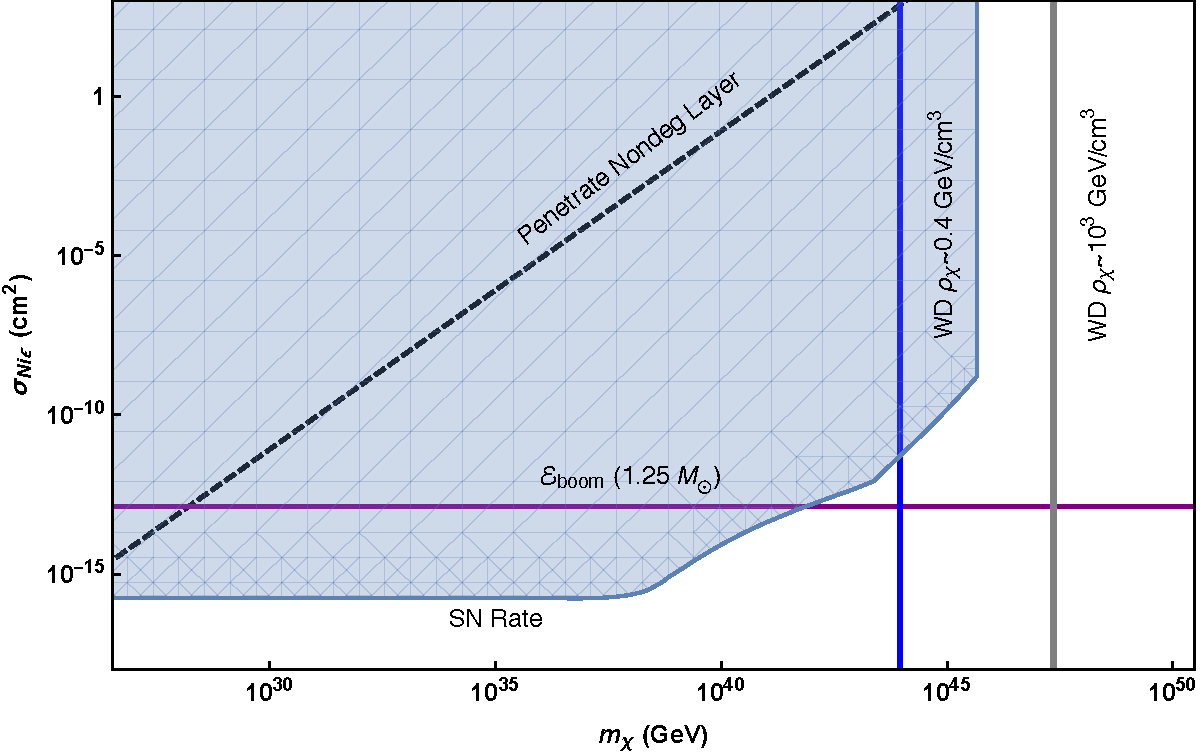
\includegraphics[scale=.35]{transitobservation.pdf}
\caption{Constraints on DM-nuclei inelastic scattering cross-section to produce a single SM product (e.g. photon) of energy $\epsilon = \text{TeV}$.
Bounds come from demanding that the DM transit triggers runaway fusion \eqref{eq:transitexplosion} (purple), occurs at a rate \eqref{eq:TransitRate} large enough to either ignite a single observed $1.25~M_{\astrosun}$ WD in its lifetime or exceed the measured SN rate in our galaxy (blue shaded). The dashed line is an example of the envelope-penetration constraint, assuming the energy deposit comes entirely from the DM's kinetic energy.
}
\label{fig:transit-inelastic}
\end{figure}

\subsection{Collision and Decay Constraints}
\label{sec:CollisionConstraints}

In order to constrain a DM model through its annihilations or decays within a WD, we require that it satisfy the ignition condition \eqref{eq:coldecay}.
Consider a simplified interaction wherein a single annihilation or decay releases $N$ particles of SM species $i$ and energy $\epsilon$.
Assuming a fractional parameter $f_\text{SM} = 1$, this corresponds to SM products with individual energy $\epsilon \sim m_\chi/N$.
Again, as long as $\epsilon \gg \MeV$ there is minimal dependence of the constraints on number of particles $N$ or species $i$ (with the exception of neutrinos).

With this schematic for the DM interaction, we can constrain the cross section for collision $\sigma_{\chi \chi}$ and lifetime $\tau_\chi$.
This is done in Figures~\ref{fig:transit-collision} and~\ref{fig:transit-decay} in the case of transiting DM using the different classes of observables for DM-DM collisions and DM decays, respectively.
In the case of captured DM, we also specify a benchmark value for the elastic scattering cross section $\sigma_{\chi A}$ and, with regards to DM-DM collisions, a stabilizing radius for the collapsing DM sphere.
This is done in Figures~\ref{fig:capture-collision} and~\ref{fig:capture-decay}---for simplicity, here we only show the constraints from the existence of nearby, heavy WDs.

\begin{figure}
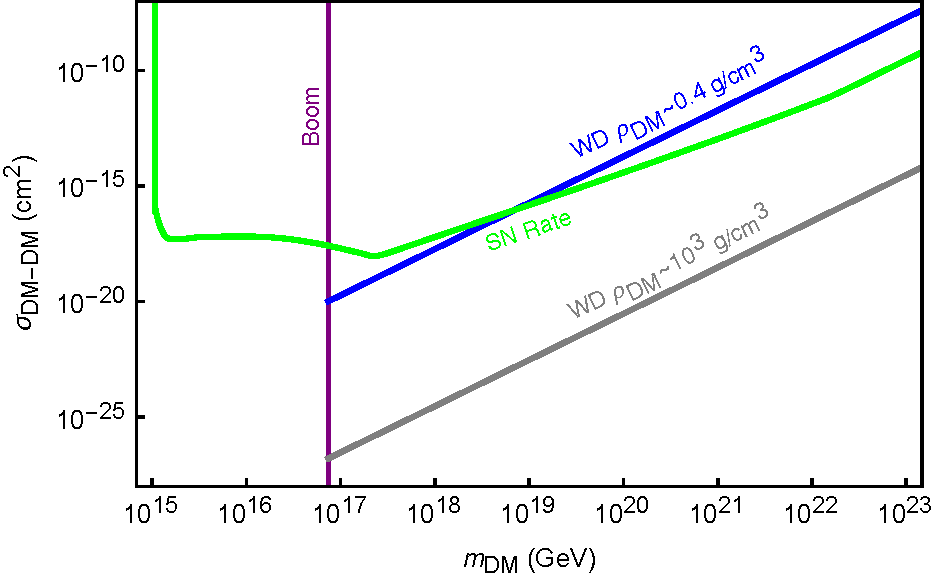
\includegraphics[scale=.35]{collisionobservation.pdf}
\caption{Constraints on DM-DM collision cross-section to SM products of energy $\epsilon \gg \MeV$.
Bounds come from demanding that the DM transit interaction triggers runaway fusion \eqref{eq:coldecay} (purple) and occurs at a rate \eqref{eq:collisionDM} large enough to either ignite a single observed $1.25~M_{\astrosun}$ WD in its lifetime or exceed the measured SN rate in our galaxy (blue shaded).
Also shown is the cosmological bound on DM self-interaction (red).}
\label{fig:transit-collision}
\end{figure}

\begin{figure}
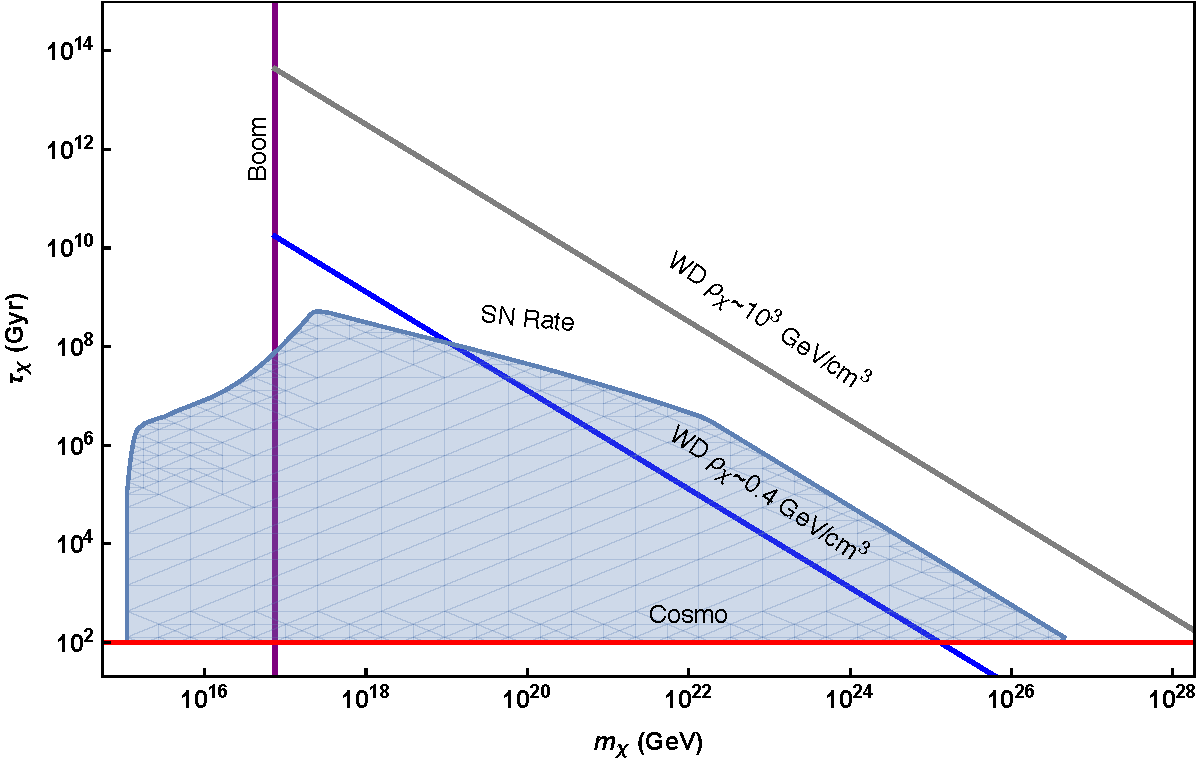
\includegraphics[scale=.35]{decayobservation.pdf}
\caption{Constraints on DM decay to SM products of energy $\epsilon \gg \MeV$.
Bounds come from demanding that the DM transit interaction triggers runaway fusion \eqref{eq:coldecay} (purple) and occurs at a rate \eqref{eq:decayDM} large enough to either ignite a single observed $1.25~M_{\astrosun}$ WD in its lifetime or exceed the measured SN rate in our galaxy (blue shaded).
Also shown is the cosmological bound on DM lifetime (red).}
\label{fig:transit-decay}
\end{figure}

\begin{figure}
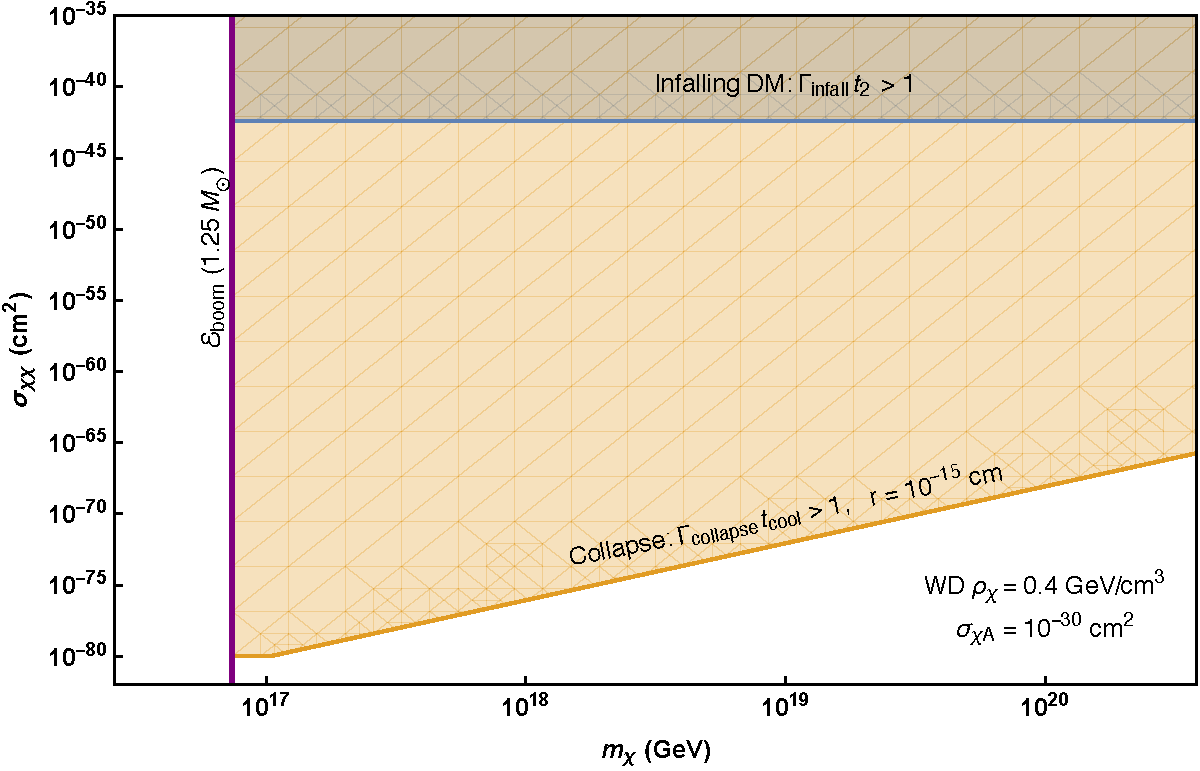
\includegraphics[scale=.35]{capturecollision.pdf}
\caption{Constraints on DM-DM collision cross-section to SM products of energy $\epsilon \gg \MeV$, assuming DM is captured with an elastic scattering $\sigma_{\chi A} = 10^{-30} ~\cm^2$.
Bounds come from the observation of a single $1.25~M_{\astrosun}$ WD in local DM density.
We consider the annihilation rate during the in-falling thermalization stage \eqref{eq:infall} (blue shaded) and during self-gravitational collapse \eqref{eq:collapse} to a stable radius $r = 10^{-15} ~\cm$ (orange shaded). See text for details.
}
\label{fig:capture-collision}
\end{figure}

\begin{figure}
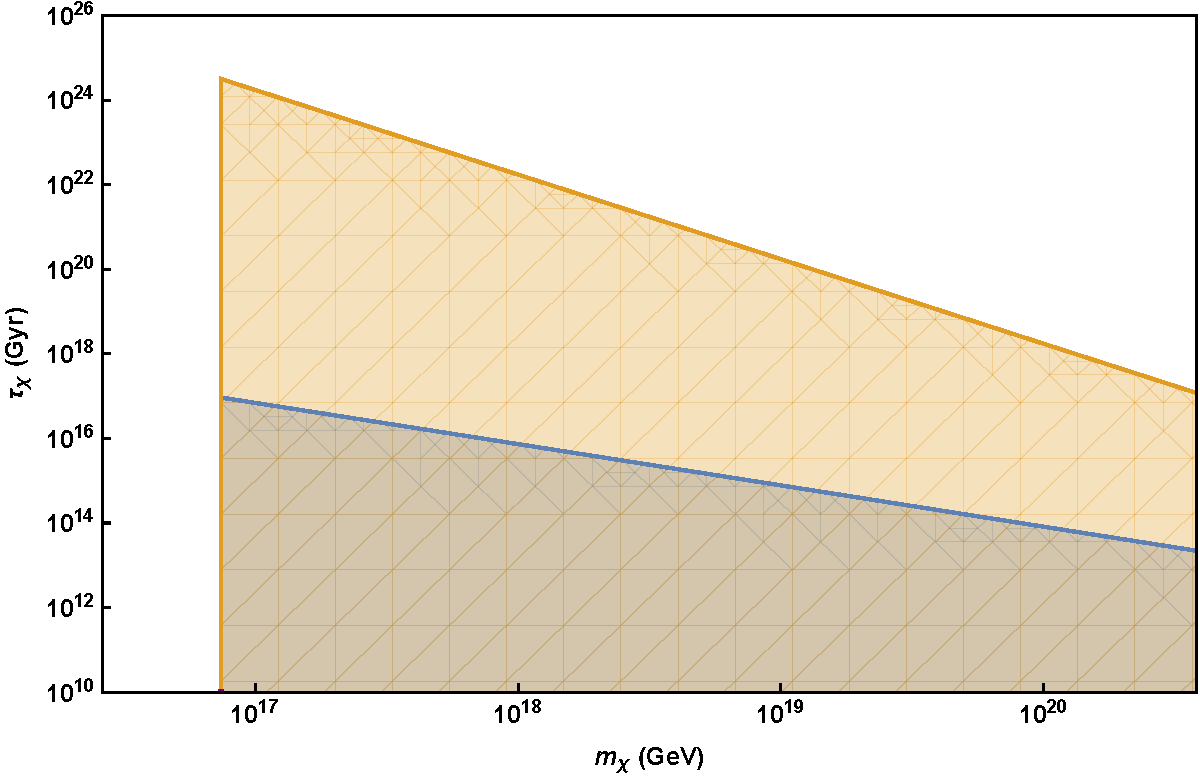
\includegraphics[scale=.35]{capturedecay.pdf}
\caption{Constraints on DM decay to SM products of energy $\epsilon \gg \MeV$, assuming DM is captured with an elastic scattering $\sigma_{\chi A} = 10^{-30} ~\cm^2$.
Bounds come from the observation of a single $1.25~M_{\astrosun}$ WD in local DM density.
We consider the decay rate during the in-falling thermalization stage \eqref{eq:decayDMcap} for gravitational collapse to a non-decaying DM core (blue shaded) or decaying DM core (orange shaded). See text for details.
}
\label{fig:capture-decay}
\end{figure}


Of course, there are additional limits on DM interactions of this kind complementary to the limits placed from WDs.
For one, demanding that the galactic halo has not substantially depleted during its lifetime yields a cosmological bound on DM self-interactions $\frac{\sigma_{\chi \chi}}{m_\chi} < \frac{\text{b}}{\GeV}$.
This is similar in magnitude to the bounds from colliding galaxy clusters \cite{Randall:2007ph}.
There is also a cosmological bound on DM lifetime $\tau_\chi > 100 ~\text{Gyr}$, independent of the nature of the decay products \cite{Poulin:2016nat}.
In addition, DM annihilations/decays in the galactic halo would contribute to the cosmic ray (CR) flux seen in terrestrial detectors.
As CRs of energy greater than $10^{12} ~\GeV$ have not yet been observed \cite{ThePierreAuger:2015rha, AbuZayyad:2012ru}, this places a bound on DM interaction parameters $\sigma_{\chi \chi}$ and $\tau_\chi$ which involve the release of such ultra-high energy particles.
The CR constraint on DM can be estimated by requiring that the expected time for an event to strike earth is less than the typical lifetime of a terrestrial detector $\sim 10 ~\text{yr}$.
For a detector of area $\sim (50~\text{km})^2$ \cite{ThePierreAuger:2015rha}, we find that the CR bounds are generally weaker than but within a few orders of magnitude of the WD bounds in the transit scenario.
This is actually due to a coincidence in the effective ``space-time volumes" of the two systems.
A CR detector sees events within a space-time volume $(R_\text{det}^2 R_\text{halo} \times 10 ~\text{yr})$ which is comparable to the WD space-time volume $(R_\text{WD}^3 \times 10^9 ~\text{yr})$, including the additional gravitational enhancement factors.
Note that a constraint can also be placed on lower-energy SM products from DM annihilations or decays which would provide an additional source for the measured CR flux, although such an analysis is beyond the scope of this work.


%%%%%%%%%%%%%%%%%%%%%%%%%%%%%%%%%%%%%%%%%%%%%%%%%%%%%%%%%%%%%%%%
\section{Q-balls}
\label{sec:qballs}
Having derived constraints on generic models of ultra-heavy DM, we turn towards a concrete example.
In various supersymmetric extensions of the SM, non-topological solitons called Q-balls can be produced in the early universe \cite{Coleman:1985ki, Kusenko:1997si}.
If these Q-balls were stable, they would comprise a component of the DM today.
For gauge-mediated models with flat scalar potentials, the Q-ball mass and radius are given by
\begin{equation}
\label{eq:Qballprop}
M_Q \sim m_S Q^{3/4}, ~~~ R_Q \sim m_S^{-1} Q^{1/4},
\end{equation}
where $m_S$ is related to the scale of supersymmetry breaking, and $Q$ is the global charge of the Q-ball---in our case, baryon number.
The condition $M_Q/Q < m_p$ ensures that the Q-ball is stable against decay to nucleons.
When an electrically neutral baryonic Q-ball interacts with a nucleon, it absorbs its baryonic charge and induces the dissociation of the nucleon into free quarks.
During this proton decay-like process, $\sim \text{GeV}$ of energy is released through the emission of 2--3 pions~\cite{Kusenko:1998}.
We assume that for each Q-ball collision, there is equal probability to produce $\pi^0$ and $\pi^\pm$ under the constraint of charge conservation.
Note that a sufficiently massive Q-ball will become a black hole if $R_Q \lesssim G M_Q$.
In the model described above, this translates into a condition $(M_\text{pl}/m_S)^4 \lesssim Q$.

We now determine the explosiveness of a Q-ball transit.
As in Section \ref{sec:Constraints}, this process is described by the parameter
\begin{equation}
\label{eq:QballLET}
\l\frac{dE}{dx}\r_\text{LET} \sim n_\text{ion} \sigma_Q N \epsilon,
\end{equation}
where the nuclear collision results in $N \sim 30$ pions released, each with kinetic energy $\epsilon \sim 500 ~\text{MeV}$.
These pions induce hadronic showers which terminate in low-energy hadrons that rapidly transfer their energy to ions via elastic scatters, as discussed in Section~\ref{sec:smheating}.
Thus the Q-ball transit has a heating length within the trigger size, and the Q-ball cross-section necessary to trigger runaway fusion is given by equations~\eqref{eq:transitexplosion} and~\eqref{eq:QballLET}:
\begin{equation}
 \sigma_Q \gtrsim \frac{1}{n_\text{ion}} \frac{\Eboom}{\lambda_T}
 \l \frac{1}{10~\GeV} \r.
\end{equation}
We see $\sigma_Q \approx 10^{-12} ~\text{cm}^2$ is sufficient to blow up a $\sim 1.25 ~M_{\astrosun}$ WD.
The cross-section for this interaction is approximately geometric
\begin{align}
\sigma_Q \sim \pi R_Q^2,
\end{align}
and so $Q \gtrsim 10^{42} ~(m_S/\text{TeV})^4$ can be adequately constrained from the observation of a single, heavy WD.
Note that the Q-ball interaction described above results in minimal slowing or transfer of kinetic energy for Q-balls this massive, so transits will easily penetrate the non-degenerate WD layer \eqref{eq:CrustCondition}.

The strongest previous constraints on Q-balls come from Super-Kamiokande as well as air fluorescence detectors of cosmic rays \cite{Dine:2003ax}.
However, the constraints due to white dwarfs are in a fundamentally complementary region of parameter space.
These are plotted in Figure~\ref{fig:Qballconstraint}.
As a comparison, the combined limits from Super-K and the OA, TA cosmic ray detectors are shown in red.
We have also included the constraints from a WD which result from considering gravitational heating during a Q-ball transit, as in \cite{Graham:2015apa}.

%%%%%%%%%%%%%%%%%%%%%%%%%%%%%%%%%%%%%%%%%%%%%%%%%%%%%%%%%%%%%%%%
\section{Discussion}
\label{sec:discussion}
The detection of ultra-heavy DM is an open problem which will likely require a confluence of astrophysical probes.
Here we present a comprehensive guide to containing these DM candidates through annihilates, decays, and transits within a WD that release sufficient SM energy to trigger a type 1a supernova.
In particular, we calculate the energy loss of high-energy particles due to SM interactions within the WD medium and determine the conditions for which a general energy deposition will heat a WD and ignite thermonuclear runaway.
The formalism provided will enable WDs to be applied as detectors for any DM models capable of heating the star through non-gravitational interactions, and as a concrete example we are able to place bounds on supersymmetric Q-ball DM over a wide region of parameter space.

In general, the phenomenology of such a DM-induced event will be the ignition of sub-Chandrasekhar mass progenitors.
This raises the tantalizing possibility that DM encounters with a WD can act as an alternative explosion mechanism and progenitor system for type 1a SN.
For decades, standard lore has been that type 1a SN are caused by accretion onto carbon-oxygen white dwarfs in binary systems that reach the critical $\sim 1.4 ~M_{\astrosun}$ Chandrasekhar mass limit.
Nevertheless, it is well-known that such a mechanism cannot account for all observed type 1a SN.
Recent observations \cite{Scalzo:2014sap, Scalzo:2014wxa} suggest that an $\OO(1)$ fraction of the observed type 1a SN appear to have sub-Chandrasekhar progenitors.
A leading explanation for this phenomenon is the detonation of a surface layer of helium which drives a shock into the interior of a sub-Chandrasekhar-mass WD \cite{Woosley1994,Fink:2007fv}.
However, in light of the lack of understanding of DM and its interactions, it is worthwhile to consider whether a DM-WD encounter may also give rise to type 1a SN progenitor.

%%%%%%%%%%%%%%%%%%%%%%%%%%%%%%%%%%%%%%%%%%%%%%%%%%%%%%%%%%%%%%%%
\begin{appendices}
\renewcommand{\thesubsection}{\arabic{subsection}}
\section{Particle Stopping in a White Dwarf}
\label{sec:wdpdg}
Here we provide a more detailed analysis of the stopping power (energy loss per distance traveled) of high-energy SM particles in a carbon-oxygen WD due to electromagnetic and strong interactions.
We consider incident electrons, photons, pions, and nucleons with kinetic energy greater than an $\MeV$.

%%%%%%%%%%%%%%%%%%%%%%%%%%%%%%%%%%%%%%%%%%%%%%%%%%%%%%%%%%%%%%%%%%%
\subsection{WD Medium}
For the WD masses that we consider, the stellar medium consists of electrons and fully-ionized carbon nuclei with densities in the range $n_e = Z n_\ion \sim 10^{31} - 10^{33} ~\cm^{-3}$ where $Z=6$.
The internal temperature is $T \sim \keV$~\cite{KippenhahnWeigert}.
The electrons are degenerate and predominantly relativistic free gas, with Fermi energy
\begin{equation}
  E_F \sim (3 \pi^2 n_e)^{1/3} \sim 1 -10 ~\MeV.
\end{equation}
The carbon ions, however, are non-degenerate and do not form a free gas. 
The plasma frequency due to ion-ion Coulomb interactions is given by
\begin{align}
\Omega_p = \l \frac{4 \pi n_\ion Z^2 \alpha}{m_\ion}\r^{1/2} \sim 1 - 10~\keV,
\end{align}
where $m_\ion$ is the ion mass.
Finally, the medium also contains thermal photons, though these are never significant for stopping particles as the photon number density $n_\gamma \sim T^3$ is much smaller than that of electrons or ions.

%%%%%%%%%%%%%%%%%%%%%%%%%%%%%%%%%%%%%%%%%%%%%%%%%%%%%%%%%%%%%%%%%%%
\subsection{Nuclear Interactions}
\label{sec:nuclear}

\paragraph{Elastic Scattering of Hadrons.}
Hadrons with energy less than $10~\MeV$ will predominantly stop due to elastic nuclear scatters with ions. 
These are hard scatters, resulting in a stopping power 
\begin{align}
  \frac{dE}{dx} \sim \frac{m}{m_\ion} E n_\ion \sigma_\el
\end{align}
for a hadron of mass $m \ll m_\ion$ and kinetic energy $E$. 
$\sigma_\el$ is the elastic nuclear scattering cross-section, which is of order $\sim \bn$ at these energies and drops to $\sim 0.1 \bn$ above $10~\MeV$~\cite{Tavernier}, ignoring the presence of various nuclear resonances in the range $1~\MeV$ to $10~\MeV$. 

\paragraph{Inelastic Scattering of Hadrons.}
For energies above $10 ~\MeV$, the stopping of hadrons is dominated by inelastic nuclear scatters.
In such a collision, an incoming hadron interacts with one or more nucleons to produce a $\OO(1)$ number of additional hadrons which approximately split the initial energy.
For incident energy greater than $\sim \GeV$, the majority of secondary hadrons are pions with transverse momenta $\sim 100 ~\MeV$ \cite{Tavernier}.
Below $\sim\GeV$, it is found that roughly equal fractions of protons, neutrons, and pions are produced in each collision \cite{Pionnuclear}.
We will thus have a roughly collinear shower terminating at an energy $\sim 10~\MeV$ which consists of pions for most of the shower's development and converts to an mix of pions and nucleons in the final decade of energy.
This cascade is described by a radiative stopping power
\begin{equation}
\label{eq:nucshower}
  \frac{dE}{dx} \sim n_\ion \sigma_\inel E,
\end{equation}
where the inelastic nuclear cross-section $\sigma_\inel$ is given by $\sigma_\inel \approx 100 ~\mbn$ and is roughly constant in energy~\cite{Tavernier}.
The total length of the shower is only logarithmically dependent on the initial hadron energy $E$,
\begin{align}
    X_\x{had} \sim \frac{1}{n_\ion \sigma_\inel} \log\l\frac{E}{10~\MeV}\r.
\end{align}

\paragraph{Photonuclear and Electronucelar Interactions.}
Photons of energy $k \gtrsim 10 ~\MeV$ can also strongly interact with nuclei through the production of virtual quark-antiquark pairs.
This destroys the photon and fragments the nucleus, producing outgoing hadrons in a manner similar to the inelastic collisions of hadrons, although the cross-section $\sigma_{\gamma A}$ is roughly a factor $\approx \alpha$ smaller.
Below $\sim \GeV$ the photonuclear cross-section is complicated by nuclear resonances while above $\sim \GeV$, $\sigma_{\gamma A}$ is a slowly increasing function of energy \cite{Tavernier}.
This increase is due to a coherent interaction of the photon over multiple nuclei at higher energies~\cite{Gerhardt:2010bj}, however instead of extrapolating this we conservatively take a constant photonuclear cross-section of order $\sigma_{\gamma A} \approx \mbn$ for energies $k \gtrsim 10 ~\MeV$.

Electrons can similarly lose energy by radiating a virtual photon that interacts hadronically with a nuclei.
The cross-section for this process is roughly given by the photonuclear cross-section and scaled by a factor representing the probability to radiate such a photon.
This is the Weizsacker-Williams approximation, which gives a cross-section for an electron of kinetic energy $E$ to exchange an energy $k$ with a nucleus
\begin{align}
    \frac{d\sigma}{dk} &\approx \frac{dN}{dk} \sigma_{\gamma A}
\end{align}
where $dN/dk$ is the virtual photon flux \cite{Gerhardt:2010bj}
\begin{align}
    \frac{dN}{dk} &\sim \frac{\alpha}{k} \log\l \frac{E}{m_e} \r.
\end{align}
Integrating this give the stopping power,
\begin{align}
    \frac{dE}{dx} &\sim n_\ion \int_{k_\xmin}^E dk \;
    k \cdot \frac{\alpha}{k} \log\l \frac{E}{m_e} \r  \sigma_{\gamma A} \\
    &\approx \alpha \log\l \frac{E}{m_e} \r \sigma_{\gamma A} n_\ion E.
\end{align}
$k_\xmin$ is taken to be the critical energy for photonuclear interactions.
Electronuclear stopping thus proceeds as a radiative process with length scale larger than the photonuclear length by a factor $\sim 10$.
Unlike the photonuclear event, this is a continuous radiative process with equal energy-loss contritions from radiation with all energies up to $E$.

%%%%%%%%%%%%%%%%%%%%%%%%%%%%%%%%%%%%%%%%%%%%%%%%%%%%%%%%%%%%%%%%%%%
\subsection{Radiative Processes}
\label{sec:emshowers}

EM showers due to successive bremsstrahlung and pair production events off carbon ions are the dominant stopping mechanisms for intermediate-energy electrons and photons.
Both of these processes result in radiative stopping powers, expressed semi-classically as~\cite{Klein:1998du} 
\begin{align}
\label{eq:SemiclassicalBrem}
  \frac{dE}{dx} \sim n_\ion \frac{Z^2 \alpha^3}{m_e^2} E \; \log{\Lambda}
\end{align}
where $\log\Lambda$ is a Coulomb form factor given by the range of effective impact parameters $b$:
\begin{align}
  \Lambda = \frac{b_\xmax}{b_\xmin} \sim \lambda_\TF m_e.
\end{align} 
The maximal impact parameter is set by the plasma screening length and the minimum by the electron mass, below which the semi-classical description breaks down. 
For the highest WD densities, we may indeed have that $\Lambda \lesssim 1$, in which case equation~\eqref{eq:SemiclassicalBrem} ought be replaced by a quantum mechanical result, such as the Bethe-Heitler formula~\cite{Bethe1934}.
This still results in a stopping power $\sim n_\ion Z^2 \alpha^3 E/m_e^2$, and so for simplicity we employ equation~\eqref{eq:SemiclassicalBrem} and take $\log{\Lambda} \sim \OO(1)$ for all WD densities.

\paragraph{LPM Suppression}
A radiative event involving momentum transfer $q$ to an ion must, quantum mechanically, occur over a length $\sim q^{-1}$. 
All ions within this region contribute to the scattering of the incident particle, and for sufficiently small $q$ this results in a decoherence that suppresses the formation of photons or electron-position pairs.
This is the ``Landau-Pomeranchuk-Midgal'' (LPM) effect. 
The momentum transfer $q$ in a given event decreases with increasing incident particle energy, and so the LPM effect will suppress radiative processes for energies greater than some scale $E_\LPM$. 
This can be calculated semi-classically~\cite{Klein:1998du}, 
\begin{align}
  E_\LPM = \frac{m_e^4}{4 \pi Z^2 \alpha^2 n_\ion}
  \approx 1~\MeV \l \frac{10^{32} \cm^{-3}}{n_\ion} \r.
\label{eq:LPM}
\end{align}
which is quite small due to the high ion density in the WD. 
The stopping power for $E > E_\LPM$ is
\begin{align}
  \l \frac{dE}{dx} \r \sim 
  n_\ion \frac{Z^2 \alpha^3}{m_e^2} E \cdot
  \l \frac{E_\LPM}{E} \r^{1/2} \label{eq:LPMBrem} 
\end{align}

In addition to the LPM effect, soft bremsstrahlung may be suppressed in a medium as the emitted photon acquires an effective mass of order the plasma frequency $\Omega_p$.
However, for high-energy electrons this dielectric suppression only introduces a minor correction to \eqref{eq:LPMBrem}, in which soft radiation is already suppressed~\cite{Klein:1998du}.

%%%%%%%%%%%%%%%%%%%%%%%%%%%%%%%%%%%%%%%%%%%%%%%%%%%%%%%%%%%%%%%%%%%
\subsection{Coulomb Scattering}
\label{sec:coulomb}

\paragraph{Scattering off Carbon Ions.}
\label{sec:coulomb_ion}
Coulomb collisions with ions provide the dominant mechanism by which electrons with energy $1~\MeV \lesssim E \lesssim 10~\MeV$ thermalize ions.
In this scenario we may treat the ions as stationary and ignore their recoil during collisions.
The ionic charge will be screened by the mobile electrons of the medium, so incident particles will scatter via a potential
\begin{align}
  \label{eq:ScreenedPotential}
V(\textbf{r}) = \frac{Z \alpha}{r} e^{-\lambda_\TF r}.
\end{align}
The screening length $\lambda_\TF$ is given in the Thomas-Fermi approximation by \cite{Teukolsky}
\begin{align}
\label{eq:TF}
    \lambda_\TF^{2} = \frac{E_F}{6 \pi \alpha n_e} 
    \sim \frac{1}{\alpha n_e^{2/3}}
\end{align}
where $E_F$ is the electron Fermi energy.
This plasma screening suppresses scatters with momentum transfers below $\sim \lambda_\TF^{-1}$, corresponding to a minimal energy transfer of $\omega_\xmin = \lambda_\TF^{-2} / 2 m_\ion$.
Ions may in principle also cause screening through lattice distortion, however this may be ignored as the sound speed of the lattice $c_s \sim 10^{-2}$ is much smaller than the speed of an incident relativistic electron. 
Using the Born approximation, we have a cross-section for energy transfer $\omega$
\begin{align}
\label{eq:CoulombOffIonsCrossSection}
  \frac{d \sigma}{d \omega} = 
  \frac{2 \pi Z^2 \alpha^2}{m_\ion\beta^2} 
  \frac{1}{(\omega + \omega_\xmin)^2}
\end{align}
and a stopping power 
\begin{align}
  \frac{dE}{d x} &= \int_{0}^{\omega_\xmax} d \omega \, n_\ion 
  \frac{d \sigma}{d \omega} \omega \nonumber\\
  \label{eq:StoppingPowerOffIons}
   &\approx \frac{2 \pi\, n_\ion Z^2 \alpha^2 }{m_\ion\beta^2} 
   \log\left( \frac{\omega_\xmax}{\omega_\xmin} \right)
\end{align}
where the second line is valid if $\omega_\xmax \gg \omega_\xmin$.
$\omega_\xmax$ is the maximum possible energy transfer. 
This may be due to 4-momentum conservation, or in the case of incident electrons, the impossibility of scattering to a final energy less than $E_F$. 
4-momentum conservation sets an upper bound $\omega_\kin$, which for a stationary target is
\begin{align}
  \omega_\kin &= \frac{2 m_\ion p^2}{m_\ion^2 + m^2 + 2E m_\ion}
\end{align}
with $p$, $E$ the incoming momentum and energy. 
The Fermi upper bound is simply $\omega_F = E - E_F$ and for incident electrons $\omega_\xmax = \min\l\omega_\kin, \omega_F\r$.

For scatters that transfer energy less than the plasma frequency $\Omega_p$, one may be concerned about phonon excitations.
We estimate this by treating each ion as an independent oscillator with frequency $\Omega_p$ (an Einstein solid) and compute the stopping power due to scatters which excite a single oscillator quanta. 
There are two key differences between this and the free ion case: incident particles must transfer an energy $\Omega_p$ and the cross-section to transfer momentum $q$ is suppressed by a factor $q^2 / 2 m_\ion\Omega_p = \omega_\x{free}/\Omega_p$. 
$\omega_\x{free}$ is the energy transfer that would accompany a free ion scatter with momentum transfer $q$. 
The resulting stopping power is unchanged from the free case~\eqref{eq:StoppingPowerOffIons}, as the increased energy transfer compensates for the suppressed cross-section:
\begin{align}
  d\sigma \cdot \omega \sim 
  d\sigma_\x{free} \frac{\omega_\x{free}}{\Omega_p} 
  \cdot \Omega_p \sim 
  d\sigma_\x{free} \cdot \omega_\x{free}.
\end{align}

Finally, we note that for more massive or more energetic incident particles the cross-section~\eqref{eq:CoulombOffIonsCrossSection} must be replaced with a more complicated expression to account for the recoil of the ion during collisions. 
In these scenarios, however, this stopping power is far subdominant to hadronic or electromagnetic showers. \\

\paragraph{Scattering off Degenerate Electrons.}
\label{sec:coulomb_elec}
The scattering of incident electrons with the degenerate electron sea determines the termination energy of electromagnetic showers, and so we focus here on that scenario. 
This calculation demands two considerations not present when scattering off ions: the targets are not stationary and they require a threshold energy transfer in order to be scattered out of the Fermi sea.
In the scenario of interest, however, these do not result in a parametrically different stopping power than was found for ions in equation~\eqref{eq:StoppingPowerOffIons}. 

For incident momenta much greater than the Fermi momentum, the relative velocity is of order the incident velocity and the deflection of the incident particle will generally be small. 
It is reasonable then that scattering proceeds, up to $\OO(1)$ factors, as though a heavy incident particle is striking a light, stationary target.  
The cross-section is then given by the usual result, 
\begin{align}
  \frac{d \sigma}{d \omega} \approx
  \frac{2 \pi \alpha^2}{E_F} \frac{1}{\omega^2},
  \label{eq:CoulombRelativisticApprox}
\end{align}
where we have accounted for the target's motion by replacing its mass with the relativistic inertia $\sqrt{m_e^2 + p^2} \approx E_F$.  We have ignored plasma screening, as Pauli-blocking will provide a more stringent cutoff on soft scatters in this case. 
Scatters which transfer an energy $\omega \leq E_F$ will have a suppressed contribution to the stopping power as they can only access a fraction of the Fermi sea. 
For incident energies $E \gg E_F$ it is sufficient to ignore these suppressed scatters, i.e.,
\begin{align}
  \frac{dE}{d x} &= \int_{E_F}^{\omega_\xmax} d \omega \, n_e 
  \frac{d \sigma}{d \omega} \omega \nonumber\\
  \label{eq:StoppingPowerOffElectrons}
   &\approx \frac{2 \pi\, n_e \alpha^2 }{E_F} 
   \log\left( \frac{\omega_\xmax}{E_F} \right)
\end{align}
where, as above, $\omega_\xmax = \min\l\omega_\kin, \omega_F\r$.
This derivation is admittedly quite heuristic, and so it has been checked with a detailed numerical calculation accounting fully for the target's motion and degeneracy.
Equation~\eqref{eq:StoppingPowerOffElectrons} is indeed a good approximation to the stopping power for incident energies larger than the Fermi energy. 

%%%%%%%%%%%%%%%%%%%%%%%%%%%%%%%%%%%%%%%%%%%%%%%%%%%%%%%%%%%%%%%%%%%
\subsection{Compton Scattering}
\label{sec:compton}
For incident photon energies less than the Fermi energy, the dominant stopping is provided by Compton scatters with degenerate electrons. 
This stopping power differs parametrically from its usual form due to the target electron motion and degeneracy.

Consider an incident photon with energy $k \leq E_F$. 
Compton scatters will only occur off electrons moving roughly collinear with the photon momentum - a head-on collision would result in an energy loss for the electron, which is forbidden by Pauli exclusion. 
In the electron rest frame these collinear scatters are Thompson-like, and so the photon energy loss is dominated by backward scatters. 
For relativistic electrons near the Fermi surface, these scatters transfer an energy
\begin{align}
  \omega \approx k \l 1 - \frac{m_e^2}{4 E_F^2} \r \sim k.
\end{align}  
The cross-section can be taken in the electron rest frame, $\sigma_T \sim \alpha^2/m_e^2$, along with an `aiming' factor $1/4\pi$ to account for the restriction to initially parallel trajectories.  
Finally, for $k \ll E_F$ only those electrons near the top of the Fermi sea are available to scatter, so the photon interacts with an effective electron density of 
\begin{align}
    n_\x{eff} = \int_{E_F - k}^{E_F} g(E) \; dE 
    \approx 3 n_e \frac{k}{E_f}
\end{align}
where $g(E)$ is the Fermi density of states. This gives a stopping power 
\begin{align}
  \frac{dk}{dx} \approx \frac{\alpha^2 n_e k^2}{m_e^2 E_F}. 
\end{align}
\section{Dark Matter Capture}
\label{sec:capture}
Here we give a more detailed discussion of DM capture and its subsequent evolution in a WD. 

\subsection{Capture Rate} 
Consider a spin-independent, elastic scattering off ions with cross section $\sigma_{\chi A}$.
For the DM to ultimately be captured, it must lose energy $\sim m_\chi v^2$, where $v$ is the DM velocity (in the rest frame of the WD) asymptotically far away.
Since typically $v \ll v_\text{esc}$, the DM has velocity $v_\text{esc}$ while in the star and must lose a fraction $(v/v_\text{esc})^2$ of its kinetic energy to become captured. 
Properly, the DM velocity is described by a boosted Maxwell distribution peaked at the galactic virial velocity $v_\text{halo} \sim 10^{-3}$.
However, this differs from the ordinary Maxwell distribution by only $\OO(1)$ factors~\cite{Gould:1987ir}, and we can approximate it by (ignoring the exponential Boltzmann tail):
\begin{equation}
\frac{dn_\chi}{dv} \approx
\begin{cases}
  \frac{\rho_\chi}{m_\chi} \l \frac{v^2}{v_\text{halo}^3} \r  & v \leq v_\text{halo} \\
  0 & v > v_\text{halo}
  \end{cases}.
\end{equation} 
The DM capture rate is given by an integral of the DM transit rate weighted by a probability for capture $P_\text{cap}$
\begin{equation}
\Gamma_\text{cap} \sim \int dv \frac{d \Gamma_\text{trans}}{dv} P_\text{cap}(v),
\end{equation}
where the (differential) transit rate is
\begin{equation}
\frac{d \Gamma_\text{trans}}{dv} \sim \frac{d n_\chi}{dv} R_\text{WD}^2 \l \frac{v_\text{esc}}{v}\r^2 v.
\end{equation}
$P_\text{cap}$ depends on both the \emph{average} number of scatters in a WD
\begin{equation}
\overbar{N}_\text{scat} \sim n_\text{ion} \sigma_{\chi A} R_\text{WD},
\end{equation}
and the number of scatters \emph{needed} for capture
\begin{equation}
N_\text{cap} \sim \text{max}\left \{1, \frac{m_\chi v^2}{m_\text{ion} v_\text{esc}^2}\right \},
\end{equation}
and is most generally expressed as a Poisson sum
\begin{equation}
P_\text{cap} = 1 - \sum^{N_\text{cap}-1}_{n=0} \exp(-\overbar{N}_\text{scat})\frac{(\overbar{N}_\text{scat})^n}{n!}.
\end{equation}
For our purposes we will approximate the sum as follows:
\begin{equation}
P_\text{cap} \approx 
\begin{cases}
 1 & \overbar{N}_\text{scat} > N_\text{cap} \\
 \overbar{N}_\text{scat} & \overbar{N}_\text{scat} < N_\text{cap} ~\text{and}~ N_\text{cap} = 1 \\
 0 & \text{else}
\end{cases}.
\end{equation}
Here we ignore the possibly of capture if $\overbar{N}_\text{scat} < N_\text{cap}$ except in the special case that only one scatter is needed for capture. 
If $\overbar{N}_\text{scat} > N_\text{cap}$, we assume all DM is captured.
Most accurately, this capture rate should be computed numerically, e.g. see~\cite{Bramante:2017xlb} for a detailed calculation. 
However with the above simplifications we find that the capture rate is of order
\begin{align}
  \Gamma_\text{cap} &\sim \Gamma_\text{trans} \cdot 
  \text{min}\left\{1, \overbar{N}_\text{scat} \text{min}\{B,1\}\right\}, \\
  B &\equiv \frac{m_\text{ion} v_\text{esc}^2}{m_\chi v_\text{halo}^2}. 
  \nonumber
\end{align}
$B$ here encodes the necessity of multiple scattering for capture. 
For ultra-heavy DM $m_\chi > 10^{15} ~\GeV$, $B \ll 1$ and essentially multiple scatters are always needed. 

To compare with existing direct detection constraints, we relate $\sigma_{\chi A}$ to the per-nucleon cross section
\begin{equation}
\sigma_{\chi A} = A^2 \l \frac{\mu_{\chi A}}{\mu_{\chi n}}\r^2 F^2(q) \sigma_{\chi n} \sim A^4 F^2(q) \sigma_{\chi n},
\end{equation}
where $F^2(q)$ is the Helm form factor~\cite{Helm:1956zz}.
For DM at the WD escape velocity, the typical momentum transfer to ions is $q \sim \mu_{\chi A} v_\text{esc} \sim 200 ~\MeV$ and the energy transfer is $q^2/m_\x{ion} \sim ~\MeV$. 
As this $q$ is less than or of order the inverse nuclear size, DM scattering off nuclei will be coherently enhanced. 
We find $F^2(q) \approx 0.1$ for $q \sim 200 ~\MeV$.  
Currently, the most stringent bound on DM spin-independent nuclear cross sections~\cite{Aprile:2017iyp} is:
\begin{align}
\label{eq:xenon}
\sigma_{\chi n} < 5 \times 10^{-46} ~\text{cm}^2 
\l \frac{m_\chi}{10^3 ~\GeV} \r.
\end{align}
It follows that for any DM candidate satisfying~\eqref{eq:xenon}, less than $1 \%$ of transiting DM is captured by the star.
Therefore, in the regime of interest the capture rate scales as 
\begin{equation}
\Gamma_\text{cap} \propto \frac{\sigma_{\chi A}}{m_\chi^2}. 
\end{equation} 

\subsection{Thermalization and Collapse} 
For the remainder of this section all numerical quantities are evaluated at a central WD density $n_\text{ion} \sim 10^{31} ~\cm^{-3}$, for which the relevant WD parameters are~\cite{cococubed}: 
\begin{align}
M_\text{WD} &\approx 1.25 ~M_{\astrosun} \nonumber \\
R_\text{WD} &\approx 4000 ~\text{km} \nonumber \\
v_\text{esc} &\approx 2 \times 10^{-2}. 
\end{align}
Depending on the context, the relevant density may be the average value which is of order $n_\text{ion} \approx 10^{30} ~\cm^{-3}$. 
We also assume a typical WD temperature $T \sim \text{keV}$.
In addition, for simplicity we take a fixed value of $\sigma_{\chi A}$ valid for the entire range of momentum transfers considered. 

Once DM is captured, it thermalizes to an average velocity
\begin{equation}
  v_\text{th} \sim \sqrt{\frac{T}{m_\chi}} 
  \approx 10^{-11} \l \frac{m_\chi}{10^{16} ~\GeV}\r^{-1/2},
\end{equation}
and settles to the thermal radius
\begin{align}
  R_\text{th} &\sim \l \frac{T}{G m_\chi \rho_\text{WD}}\r^{1/2} \\
 &\approx 0.1 ~\cm \l \frac{m_\chi}{10^{16} ~\GeV}\r^{-1/2}, \nonumber
\end{align}
where its kinetic energy balances against the gravitational potential energy of the (enclosed) WD mass. 
This thermalization time can be explicitly calculated for elastic nuclear scatters~\cite{Kouvaris:2010jy}. 
The stopping power due to such scatters is
\begin{align}
    \frac{dE}{dx} \sim \rho_\text{WD} \sigma_{\chi A} \; v \; \text{max}\{v, v_\ion\},
\end{align}
where $v_\ion \sim \sqrt{\frac{T}{m_\text{ion}}}$ is the thermal ion velocity. 
The max function indicates the transition between ``viscous" and ``inertial" drag. 
The DM first passes through the WD many times on a wide orbit until the size of its orbit decays to become contained in the star.
The timescale for this process is
\begin{align}
  t_1 &\sim \l \frac{m_\chi}{m_\text{ion}} \r^{3/2} 
  \frac{R_\text{WD}}{v_\text{esc}} \frac{1}{\overbar{N}_\text{scat}} 
  \frac{1}{\text{max}\{\overbar{N}_\text{scat}, 1\}^{1/2}} \\
  &\approx 7 \times 10^{16}~\text{s} \l \frac{m_\chi}{10^{16} ~\GeV} \r^{3/2} 
  \l \frac{\sigma_{\chi A}}{10^{-35} ~\cm^2} \r^{-3/2}. \nonumber
\end{align}
Subsequently, the DM completes many orbits within the star until dissipation further reduces the orbital size to the thermal radius.
The timescale for this process is
\begin{align}
  t_2  &\sim \l \frac{m_\chi}{m_\text{ion}} \r 
  \frac{1}{n_\text{ion} \sigma_{\chi A}} \frac{1}{v_\text{ion}} \\
  &\approx 10^{14}~\text{s}\l \frac{m_\chi}{10^{16} ~\GeV} \r 
  \l \frac{\sigma_{\chi A}}{10^{-35} ~\cm^2} \r^{-1}. \nonumber
\end{align}
There is an additional $\OO(10)$ logarithmic enhancement of the timescale once the DM velocity has slowed below $v_\ion$. 
Note that the two thermalization timescales are much larger than the gravitational free-fall timescale, which is the time to complete a single orbit:
\begin{equation}
\label{eq:freefalltime}
t_\text{ff} \sim \sqrt{\frac{1}{G \rho_\text{WD}}} \approx 0.5 ~\text{s}.
\end{equation}

The DM will begin steadily accumulating at $R_\text{th}$ after a time $t_1 + t_2$.
Once the collected mass of DM at the thermal radius exceeds the WD mass within this volume, there is the possibility of self-gravitational collapse.
The time to collect a critical number of DM particles is 
\begin{align}
\label{eq:Ncore}
    t_\text{sg} &\sim 
    \frac{\rho_\text{WD} R^3_\text{th}}{m_\chi \Gamma_\text{cap}} \\
    &\approx 10^{10} ~\text{s} \l \frac{m_\chi}{10^{16} ~\GeV} \r^{-1/2} 
    \l \frac{\sigma_{\chi A}}{10^{-35} ~\cm^2} \r^{-1}, \nonumber 
\end{align}
which in the regime of ultra-heavy DM is much smaller than the decay and thermalization scales $t_1$ and $t_2$.
Typically, the timescale for collapse is set by the DM sphere's ability to cool and shed gravitational potential energy.
This is initially just $t_2$, while the time to collapse at any given radius $r$ decreases once the DM velocity rises again above $v_\ion$
\begin{align}
  t_\text{cool} &\sim t_2 \text{min}\{v_\text{ion}/v_\chi,1\} \\
  v_\chi &\sim \sqrt{\frac{G N m_\chi}{r}}, \nonumber
\end{align}
where $N$ is the number of collapsing DM particles. 
However, since the DM collection timescale is shorter than the cooling time $t_\text{sg} < t_2$, the dynamics of the collapse is initially set by further collection and adiabatic shrinking of the DM sphere. 
This over-collection will necessarily increase the number of collapsing DM particles beyond $\Gamma_\text{cap} t_\text{sg}$ and hasten the collapse until the collection time matches the cooling time.
\end{appendices}

%%%%%%%%%%%%%%%%%%%%%%%%%%%%%%%%%%%%%%%%%%%%%%%%%%%%%%%%%%%%%%%%
\section*{Acknowledgements}
We would like to thank Kim Berghaus, Kyle Boone, Jeff Dror, Keisuke Harigaya, David E. Kaplan, Spencer Klein, Chris Kouvaris, Jacob Leedom, Junsong Lin, Chung-Pei Ma, Sam McDermott, Katelin Schutz, Peter Tinyakov, and Lian-Tao Wang for stimulating discussions.

%%%%%%%%%%%%%%%%%%%%%%%%%%%%%%%%%%%%%%%%%%%%%%%%%%%%%%%%%%%%%%%%
\begin{thebibliography}{99}
\bibliographystyle{unsrt}
%\cite{Graham:2015apa}
\bibitem{Graham:2015apa} 
  P.~W.~Graham, S.~Rajendran and J.~Varela,
  %``Dark Matter Triggers of Supernovae,''
  Phys.\ Rev.\ D {\bf 92}, no. 6, 063007 (2015)
  %doi:10.1103/PhysRevD.92.063007
  [arXiv:1505.04444 [hep-ph]].
  %%CITATION = doi:10.1103/PhysRevD.92.063007;%%
  %40 citations counted in INSPIRE as of 01 Mar 2018


%\cite{Akerib:2016vxi}
\bibitem{Akerib:2016vxi} 
  D.~S.~Akerib {\it et al.} [LUX Collaboration],
  %``Results from a search for dark matter in the complete LUX exposure,''
  Phys.\ Rev.\ Lett.\  {\bf 118}, no. 2, 021303 (2017)
  %doi:10.1103/PhysRevLett.118.021303
  [arXiv:1608.07648 [astro-ph.CO]].
  %%CITATION = doi:10.1103/PhysRevLett.118.021303;%%
  %555 citations counted in INSPIRE as of 01 Mar 2018


%\cite{Agnese:2017njq}
\bibitem{Agnese:2017njq} 
  R.~Agnese {\it et al.} [SuperCDMS Collaboration],
  %``Results from the Super Cryogenic Dark Matter Search Experiment at Soudan,''
  Phys.\ Rev.\ Lett.\  {\bf 120}, no. 6, 061802 (2018)
  %doi:10.1103/PhysRevLett.120.061802
  [arXiv:1708.08869 [hep-ex]].
  %%CITATION = doi:10.1103/PhysRevLett.120.061802;%%
  %8 citations counted in INSPIRE as of 01 Mar 2018


%\cite{Griest:2013aaa}
\bibitem{Griest:2013aaa} 
  K.~Griest, A.~M.~Cieplak and M.~J.~Lehner,
  %``Experimental Limits on Primordial Black Hole Dark Matter from the First 2 yr of Kepler Data,''
  Astrophys.\ J.\  {\bf 786}, no. 2, 158 (2014)
  %doi:10.1088/0004-637X/786/2/158
  [arXiv:1307.5798 [astro-ph.CO]].
  %%CITATION = doi:10.1088/0004-637X/786/2/158;%%
  %54 citations counted in INSPIRE as of 01 Mar 2018


%\cite{Scalzo:2014sap}
\bibitem{Scalzo:2014sap} 
  R.~Scalzo {\it et al.} [Nearby Supernova Factory Collaboration],
  %``Type Ia supernova bolometric light curves and ejected mass estimates from the Nearby Supernova Factory,''
  Mon.\ Not.\ Roy.\ Astron.\ Soc.\  {\bf 440}, no. 2, 1498 (2014)
  %doi:10.1093/mnras/stu350
  [arXiv:1402.6842 [astro-ph.CO]].
  %%CITATION = doi:10.1093/mnras/stu350;%%
  %40 citations counted in INSPIRE as of 01 Mar 2018


%\cite{Scalzo:2014wxa}
\bibitem{Scalzo:2014wxa} 
  R.~A.~Scalzo, A.~J.~Ruiter and S.~A.~Sim,
  %``The ejected mass distribution of type Ia supernovae: A significant rate of non-Chandrasekhar-mass progenitors,''
  Mon.\ Not.\ Roy.\ Astron.\ Soc.\  {\bf 445}, no. 3, 2535 (2014)
  %doi:10.1093/mnras/stu1808
  [arXiv:1408.6601 [astro-ph.HE]].
  %%CITATION = doi:10.1093/mnras/stu1808;%%
  %40 citations counted in INSPIRE as of 01 Mar 2018


\bibitem{Woosley1994}
  %Sub--Chandrasekhar Mass Models for type 1a Supernovae
  S.~E.~Woosley and T.~A.~Weaver, Astrophysical Journal {\bf 423}, pp.371-379 (1994).

%\cite{Fink:2007fv}
\bibitem{Fink:2007fv} 
  M.~Fink, W.~Hillebrandt and F.~K.~Roepke,
  %``Double-detonation supernovae of sub-Chandrasekhar mass white dwarfs,''
  Astron.\ Astrophys.\ 
  [Astron.\ Astrophys.\  {\bf 476}, 1133 (2007)]
  %doi:10.1051/0004-6361:20078438
  [arXiv:0710.5486 [astro-ph]].
  %%CITATION = doi:10.1051/0004-6361:20078438;%%
  %74 citations counted in INSPIRE as of 01 Mar 2018


%\cite{Pakmor:2013wia}
\bibitem{Pakmor:2013wia} 
  R.~Pakmor, M.~Kromer and S.~Taubenberger,
  %``Helium-ignited violent mergers as a unified model for normal and rapidly declining Type Ia Supernovae,''
  Astrophys.\ J.\  {\bf 770}, L8 (2013)
  %doi:10.1088/2041-8205/770/1/L8
  [arXiv:1302.2913 [astro-ph.HE]].
  %%CITATION = doi:10.1088/2041-8205/770/1/L8;%%
  %69 citations counted in INSPIRE as of 01 Mar 2018


\bibitem{Woosley}
 F.~X. Timmes and S.~E. Woosley, Astro. Phys. Journal {\bf 396}, 649 (1992).

%\cite{Gasques:2005ar}
\bibitem{Gasques:2005ar} 
  L.~R.~Gasques, A.~V.~Afanasjev, E.~F.~Aguilera, M.~Beard, L.~C.~Chamon, P.~Ring, M.~Wiescher and D.~G.~Yakovlev,
  %``Nuclear fusion in dense matter: Reaction rate and carbon burning,''
  Phys.\ Rev.\ C {\bf 72}, 025806 (2005)
  %doi:10.1103/PhysRevC.72.025806
  [astro-ph/0506386].
  %%CITATION = doi:10.1103/PhysRevC.72.025806;%%
  %62 citations counted in INSPIRE as of 01 Mar 2018


\bibitem{cococubed}
F.~X.~Timmes, \href{http://cococubed.asu.edu/code_pages/coldwd.shtml}{link}

%\cite{Gandhi:1998ri}
\bibitem{Gandhi:1998ri} 
  R.~Gandhi, C.~Quigg, M.~H.~Reno and I.~Sarcevic,
  %``Neutrino interactions at ultrahigh-energies,''
  Phys.\ Rev.\ D {\bf 58}, 093009 (1998)
  %doi:10.1103/PhysRevD.58.093009
  [hep-ph/9807264].
  %%CITATION = doi:10.1103/PhysRevD.58.093009;%%
  %626 citations counted in INSPIRE as of 01 Mar 2018


%\cite{Formaggio:2013kya}
\bibitem{Formaggio:2013kya} 
  J.~A.~Formaggio and G.~P.~Zeller,
  %``From eV to EeV: Neutrino Cross Sections Across Energy Scales,''
  Rev.\ Mod.\ Phys.\  {\bf 84}, 1307 (2012)
  %doi:10.1103/RevModPhys.84.1307
  [arXiv:1305.7513 [hep-ex]].
  %%CITATION = doi:10.1103/RevModPhys.84.1307;%%
  %233 citations counted in INSPIRE as of 01 Mar 2018


\bibitem{KippenhahnWeigert}
R.~Kippenhahn and A.~Weigert, "Stellar Structure and Evolution, Springer (1994).

%\cite{Press:1985ug}
\bibitem{Press:1985ug} 
  W.~H.~Press and D.~N.~Spergel,
  %``Capture by the sun of a galactic population of weakly interacting massive particles,''
  Astrophys.\ J.\  {\bf 296}, 679 (1985).
  %doi:10.1086/163485
  %%CITATION = doi:10.1086/163485;%%
  %457 citations counted in INSPIRE as of 01 Mar 2018


%\cite{Gould:1987ir}
\bibitem{Gould:1987ir} 
  A.~Gould,
  %``Resonant Enhancements in WIMP Capture by the Earth,''
  Astrophys.\ J.\  {\bf 321}, 571 (1987).
  %doi:10.1086/165653
  %%CITATION = doi:10.1086/165653;%%
  %441 citations counted in INSPIRE as of 01 Mar 2018


%\cite{Aprile:2017iyp}
\bibitem{Aprile:2017iyp} 
  E.~Aprile {\it et al.} [XENON Collaboration],
  %``First Dark Matter Search Results from the XENON1T Experiment,''
  Phys.\ Rev.\ Lett.\  {\bf 119}, no. 18, 181301 (2017)
  %doi:10.1103/PhysRevLett.119.181301
  [arXiv:1705.06655 [astro-ph.CO]].
  %%CITATION = doi:10.1103/PhysRevLett.119.181301;%%
  %269 citations counted in INSPIRE as of 01 Mar 2018

\bibitem{us}
R.~Janish, V.~Narayan, and P.~Riggins, in preparation

%\cite{Mereghetti:2013nba}
\bibitem{Mereghetti:2013nba} 
  S.~Mereghetti,
  %``RX J0648.0--4418: the fastest-spinning white dwarf,''
  %doi:10.1142/9789814623995_0469
  arXiv:1302.4634 [astro-ph.HE].
  %%CITATION = doi:10.1142/9789814623995_0469;%%
  %3 citations counted in INSPIRE as of 01 Mar 2018


\bibitem{SDSS}
S.~J.~Kleinman, S. O. Kepler, D. Koester, I. Pelisoli  {\it et al.}, Astrophys. J. Suppl. {\bf 204}, article
id. 5, 14 pp. (2013)

\bibitem{NuStar}
K.~Perez, C.~J.~Hailey, F.~E.~Bauer, {\it et al.}, Nature {\bf 520}, 646 (2015)

%\cite{Nesti:2013uwa}
\bibitem{Nesti:2013uwa} 
  F.~Nesti and P.~Salucci,
  %``The Dark Matter halo of the  Milky Way, AD 2013,''
  JCAP {\bf 1307}, 016 (2013)
  %doi:10.1088/1475-7516/2013/07/016
  [arXiv:1304.5127 [astro-ph.GA]].
  %%CITATION = doi:10.1088/1475-7516/2013/07/016;%%
  %119 citations counted in INSPIRE as of 01 Mar 2018


\bibitem{Chandrasekhar}
S.~Chandrasekhar, ``An Introduction to the Study of Stellar Structure", University of Chicago press (1939).

%\cite{Randall:2007ph}
\bibitem{Randall:2007ph} 
  S.~W.~Randall, M.~Markevitch, D.~Clowe, A.~H.~Gonzalez and M.~Bradac,
  %``Constraints on the Self-Interaction Cross-Section of Dark Matter from Numerical Simulations of the Merging Galaxy Cluster 1E 0657-56,''
  Astrophys.\ J.\  {\bf 679}, 1173 (2008)
  %doi:10.1086/587859
  [arXiv:0704.0261 [astro-ph]].
  %%CITATION = doi:10.1086/587859;%%
  %358 citations counted in INSPIRE as of 01 Mar 2018


%\cite{Poulin:2016nat}
\bibitem{Poulin:2016nat} 
  V.~Poulin, P.~D.~Serpico and J.~Lesgourgues,
  %``A fresh look at linear cosmological constraints on a decaying dark matter component,''
  JCAP {\bf 1608}, no. 08, 036 (2016)
  %doi:10.1088/1475-7516/2016/08/036
  [arXiv:1606.02073 [astro-ph.CO]].
  %%CITATION = doi:10.1088/1475-7516/2016/08/036;%%
  %32 citations counted in INSPIRE as of 01 Mar 2018


%\cite{ThePierreAuger:2015rha}
\bibitem{ThePierreAuger:2015rha} 
  A.~Aab {\it et al.} [Pierre Auger Collaboration],
  %``Measurement of the cosmic ray spectrum above 4 $\times$ 10$^{18}$ eV using inclined events detected with the Pierre Auger Observatory,''
  JCAP {\bf 1508}, 049 (2015)
  %doi:10.1088/1475-7516/2015/08/049
  [arXiv:1503.07786 [astro-ph.HE]].
  %%CITATION = doi:10.1088/1475-7516/2015/08/049;%%
  %30 citations counted in INSPIRE as of 01 Mar 2018


%\cite{AbuZayyad:2012ru}
\bibitem{AbuZayyad:2012ru} 
  T.~Abu-Zayyad {\it et al.} [Telescope Array Collaboration],
  %``The Cosmic Ray Energy Spectrum Observed with the Surface Detector of the Telescope Array Experiment,''
  Astrophys.\ J.\  {\bf 768}, L1 (2013)
  %doi:10.1088/2041-8205/768/1/L1
  [arXiv:1205.5067 [astro-ph.HE]].
  %%CITATION = doi:10.1088/2041-8205/768/1/L1;%%
  %215 citations counted in INSPIRE as of 01 Mar 2018


%\cite{Coleman:1985ki}
\bibitem{Coleman:1985ki} 
  S.~R.~Coleman,
  %``Q Balls,''
  Nucl.\ Phys.\ B {\bf 262}, 263 (1985)
  Erratum: [Nucl.\ Phys.\ B {\bf 269}, 744 (1986)].
  %doi:10.1016/0550-3213(85)90286-X, 10.1016/0550-3213(86)90520-1
  %%CITATION = doi:10.1016/0550-3213(85)90286-X, 10.1016/0550-3213(86)90520-1;%%
  %696 citations counted in INSPIRE as of 01 Mar 2018


%\cite{Kusenko:1997si}
\bibitem{Kusenko:1997si} 
  A.~Kusenko and M.~E.~Shaposhnikov,
  %``Supersymmetric Q balls as dark matter,''
  Phys.\ Lett.\ B {\bf 418}, 46 (1998)
  %doi:10.1016/S0370-2693(97)01375-0
  [hep-ph/9709492].
  %%CITATION = doi:10.1016/S0370-2693(97)01375-0;%%
  %459 citations counted in INSPIRE as of 01 Mar 2018


\bibitem{Kusenko:1998}
  A.~Kusenko, V.~Kuzmin, M.~Shaposhnikov, P.~G.~Tinyakov,
  %``Experimental Signatures of Supersymmetric Dark-Matter $\mathit{Q}$-Balls,''
  Phys.\ Rev.\ Lett.\ {\bf 80}, 15 (1998)
  [hep-ph//9712212].

%\cite{Dine:2003ax}
\bibitem{Dine:2003ax} 
  M.~Dine and A.~Kusenko,
  %``The Origin of the matter - antimatter asymmetry,''
  Rev.\ Mod.\ Phys.\  {\bf 76}, 1 (2003)
  %doi:10.1103/RevModPhys.76.1
  [hep-ph/0303065].
  %%CITATION = doi:10.1103/RevModPhys.76.1;%%
  %394 citations counted in INSPIRE as of 01 Mar 2018


\bibitem{Tavernier}
S.~Tavernier, "Experimental Techniques in Nuclear and Particle Physics", Springer (2010).

\bibitem{Pionnuclear}
T.~S.~H.~Lee and R.~P.~Redwine,
 %``Pion-Nucleus Interactions",
 Annu. Rev. Nucl. Part. Sci {\bf 52}, pp.23-63 (2002)

%\cite{Gerhardt:2010bj}
\bibitem{Gerhardt:2010bj} 
  L.~Gerhardt and S.~R.~Klein,
  %``Electron and Photon Interactions in the Regime of Strong LPM Suppression,''
  Phys.\ Rev.\ D {\bf 82}, 074017 (2010)
  %doi:10.1103/PhysRevD.82.074017
  [arXiv:1007.0039 [hep-ph]].
  %%CITATION = doi:10.1103/PhysRevD.82.074017;%%
  %26 citations counted in INSPIRE as of 01 Mar 2018


%\cite{Klein:1998du}
\bibitem{Klein:1998du} 
  S.~Klein,
  %``Suppression of Bremsstrahlung and pair production due to environmental factors,''
  Rev.\ Mod.\ Phys.\  {\bf 71}, 1501 (1999)
  %doi:10.1103/RevModPhys.71.1501
  [hep-ph/9802442].
  %%CITATION = doi:10.1103/RevModPhys.71.1501;%%
  %156 citations counted in INSPIRE as of 01 Mar 2018


\bibitem{Bethe1934}
  H.~Bethe and W.~Heitler
  % On the stopping of fast particles and on the creation of positive electrons
  Proc.\ R.\ Soc.\ Lond.\ A 1934 146 83-112
  % doi:10.1098/rspa.1934.0140
  % http://rspa.royalsocietypublishing.org/content/146/856/83

\bibitem{Teukolsky}
S.~L.~Shapiro and S.~A.~Teukolsky, ``Black Holes, White Dwarfs, and Neutron Stars", Wiley (1983).

\bibitem{Jackson}
J.~D.~Jackson, ``Classical Electrodynamics", 3rd edition, John Wiley and Sons, New
York, (1998).

\bibitem{Rossi}
B.~Rossi, ``High Energy Particles", Prentice-Hall, Inc., Englewood Cliffs, NJ (1952).

%\cite{Bramante:2017xlb}
\bibitem{Bramante:2017xlb} 
  J.~Bramante, A.~Delgado and A.~Martin,
  %``Multiscatter stellar capture of dark matter,''
  Phys.\ Rev.\ D {\bf 96}, no. 6, 063002 (2017)
  %doi:10.1103/PhysRevD.96.063002
  [arXiv:1703.04043 [hep-ph]].
  %%CITATION = doi:10.1103/PhysRevD.96.063002;%%
  %5 citations counted in INSPIRE as of 01 Mar 2018


%\cite{Helm:1956zz}
\bibitem{Helm:1956zz} 
  R.~H.~Helm,
  %``Inelastic and Elastic Scattering of 187-Mev Electrons from Selected Even-Even Nuclei,''
  Phys.\ Rev.\  {\bf 104}, 1466 (1956).
  %doi:10.1103/PhysRev.104.1466
  %%CITATION = doi:10.1103/PhysRev.104.1466;%%
  %355 citations counted in INSPIRE as of 01 Mar 2018


%\cite{Kouvaris:2010jy}
\bibitem{Kouvaris:2010jy} 
  C.~Kouvaris and P.~Tinyakov,
  %``Constraining Asymmetric Dark Matter through observations of compact stars,''
  Phys.\ Rev.\ D {\bf 83}, 083512 (2011)
  %doi:10.1103/PhysRevD.83.083512
  [arXiv:1012.2039 [astro-ph.HE]].
  %%CITATION = doi:10.1103/PhysRevD.83.083512;%%
  %63 citations counted in INSPIRE as of 01 Mar 2018

\end{thebibliography}

\end{document}
